\documentclass[english,10pt,titlepage]{article}
\usepackage{graphicx}
\usepackage{graphics}
\usepackage{epsfig}
\usepackage{amsmath}
\usepackage{amssymb}
\usepackage{amsthm}
\usepackage[geometry]{ifsym}
\usepackage{booktabs}
\usepackage{stmaryrd}
\usepackage{color}
\usepackage{url}
\usepackage{longtable}
\usepackage[figuresright]{rotating}
\usepackage[cp1250]{inputenc}
\usepackage[T1]{fontenc}
\usepackage{babel}
\usepackage{geometry}
\usepackage{subfig}
\usepackage{pslatex}
\usepackage{ulem}
\usepackage{lipsum}
\usepackage{listings}
\usepackage{float}

\definecolor{mygreen}{RGB}{34,177,76}
\definecolor{mygrey}{RGB}{240,240,240}

\lstset{
	language=C++,
	basicstyle=\footnotesize,
	numbers=left,
	numberstyle=\footnotesize,
	keywordstyle=\color{blue},
	commentstyle=\color{mygreen},
	stepnumber=1,
	numbersep=5pt,
	backgroundcolor=\color{mygrey},
	showspaces=false,
	showstringspaces=false,
	showtabs=false,
	frame=single,
	tabsize=2,
	captionpos=b,
	breaklines=true,
	breakatwhitespace=false,
	title=\lstname,
	%escapeinside={\%*}{*)},
	morekeywords={and,or,distance,to,uniform,sampler2D,float3,float4,float3x3,float4x4,mul,POSITION,NORMAL,TEXCOORD0}
}

\setcounter{secnumdepth}{3}



\begin{document}



\pagestyle{empty}



\begin{titlepage}
\vspace*{\fill}
\begin{center}
\begin{picture}(300,510)
  \put( -10,520){\makebox(0,0)[l]{\large \bf \textsc{Faculty of Fundamental Problems of Technology}}}
  \put( -10,500){\makebox(0,0)[l]{\large \bf \textsc{Wroc�aw University of Technology}}}
  \put( 20,340){\makebox(0,0)[l]{\Huge  \bf \textsc{Software Renderer}}}
  \put( -67,300){\makebox(0,0)[l]{\Huge  \bf \textsc{Accelerated by CUDA Technology}}}
  \put(140,260){\makebox(0,0)[l]{\large     \textsc{v1.1}}}
  \put(100,220){\makebox(0,0)[l]{\large     \textsc{Wojciech Sterna}}}

  \put(170, 80){\makebox(0,0)[l]{\large  {B.Sc. Thesis written}}}
  \put(170, 60){\makebox(0,0)[l]{\large  {under the supervision of}}}
  \put(170, 40){\makebox(0,0)[l]{\large  {Marcin Zawada, Ph.D.}}}

  \put(110,-80){\makebox(0,0)[bl]{\large \bf \textsc{Wroc�aw 2011}}}
\end{picture}
\end{center}
\vspace*{\fill}
\end{titlepage}

\newpage



%\mbox{}

%\newpage



\section*{Abstract}

NVIDIA's CUDA technology allows for massively parallel and general-purpose code execution on GPU. One of the most common applications of parallelism is graphics processing. Although there are APIs that allow for extremely fast hardware graphics processing (like OpenGL or Direct3D), inherently they suffer from lack of full programmability. The goal of this work is implementation of a software renderer using CUDA technology and comparing its performance with that from fully hardwared one.

\newpage



%\mbox{}

%\newpage



\tableofcontents

\newpage



%\mbox{}

%\newpage



\pagestyle{headings}



\section{Introduction}

This section starts with discussion of basic concepts that must be known to be able to fully understand this work. Finally, goals of the project are discussed.

\subsection{Fundamental Concepts}

\begin{itemize}
	\item raster image -- a 2-dimensional array of pixels, where each pixel contains an $n$-bit value. Raster image is usually used to store colors in its pixel values but in general this can be any kind of data.
	\item rendering -- process of generating a raster image from a scene containing 3-dimensional objects from a fixed viewpoint defined by a virtual camera. Computer programs for rendering are usually referred to as renderers. Rendering techniques can be divided in two categories:
		\begin{itemize}
			\item image-order -- images rendered with this set of techniques all follow the general rule: \\ \verb|for every pixel: find object that covers it|. Good time complexity. Ray-tracing is one of the techniques that generates images this way.
			\item object-order -- images rendered with this set of techniques all follow the general rule: \\ \verb|for every object: find pixels that are covered by it|. Time complexity is worse than in image-order rendering but in practice object-order renderers appear to be faster. OpenGL and Direct3D, the most popular graphics APIs for generating images in real-time, both perform object-order rendering.
		\end{itemize}
	\item the graphics pipeline -- set of stages that input graphics data is passed through to perform rendering. Stages are usually introduced in a way that makes better understanding of how an output image is generated. The graphics pipeline, in terms of this project, will be investigated in details in chapter \ref{section:the_graphics_pipeline}.
	\item CUDA -- technology developed by NVIDIA destined for parallel, general-purpose code execution by using GPU (graphics processing unit). If a problem requires solving many instances of the same task (where all instances are independent from each other), then it can greatly benefit from CUDA. A trivial example can be geometry vertex processing, where processing of one vertex does not influence processing of any other vertex. This way many vertices can be handled at the same time.
\end{itemize}

It is assumed that the reader has a good understanding of fundamentals of analytical geometry (lines, planes), linear algebra (vectors, matrices) and calculus (partial derivatives).

\subsection{Hardware and Software Rendering}

An important thing is distinction between hardware and software renderers. The former ones use dedicated hardware to perform rendering, whereas the latter are hardware independent. A deeper discussion about both categories will take place now.

Hardware renderers, as they use dedicated hardware, are very fast in performing graphics related work so they can be used in real-time applications. The two main APIs that let a programmer make use of hardware rendering are Direct3D and OpenGL. Direct3D is being developed strictly by Microsoft and is available only on Windows, Xbox and Xbox 360. On the other hand OpenGL is under development of Khronos Group, which is a consortium formed of several corporations related to computer graphics, such as Intel, NVIDIA or ATI. The greatest advantage of OpenGL over Direct3D is that it is an open standard and is supported by various operating systems (Windows, Linux, Mac OS). Both libraries offer very similar functionality and differ only in a way they exhibit it. This functionality is dependent on hardware that is being used and as such Direct3D and OpenGL cannot go beyond a fixed set of available capabilities (the graphics pipeline is more or less fixed, thus it was called the fixed-function pipeline). Although today's graphics hardware is programmable to some point by so-called shader programs, it will never reach a point of full programmability.

Software renderers, on the other hand, are hardware independent since the code is usually executed on general-purpose processors, rather than dedicated hardware. As such software renderers do not make use of any specialized acceleration and thus are very slow. Important thing to note is that software renderers, just as hardware ones, also process geometry in some fixed way via the graphics pipeline. However, it is this graphics pipeline that can be modified in software renderers by a programmer at any time to fit new needs. In case of hardware renderers the graphics pipeline can only be modified by GPUs (graphics processing units) manufacturers.

\subsubsection{Shaders}

A few words should be said about shaders. A shader is a small computer program that is executed on the graphics card. As mentioned in the previous section, shaders introduce some level of programmability to hardware renderers. The two most recognized shader types are vertex and pixel shaders. Vertex shader is responsible for processing at the level of a single vertex, whereas pixel shader is run for all pixels of a single polygon.

Listings \ref{listing:vertex_shader} and \ref{listing:pixel_shader} present example vertex and pixel shaders. The vertex shader simply transforms vertex position and its normal vector and the job of the pixel shader is to visualize the transformed normal vector.

\begin{lstlisting}[numbers=none, label=listing:vertex_shader, caption={A simple vertex shader.}]
...

VS_OUTPUT main(VS_INPUT input)
{
	VS_OUTPUT output;

	// world-space
	float4 position = mul(input.position, worldTransform);
	float3 normal = mul(input.normal, (float3x3)worldTransform);

	output.position = mul(position, viewProjTransform);
	output.normal = normal;

	return output;
}
\end{lstlisting}

\begin{lstlisting}[numbers=none, label=listing:pixel_shader, caption={A simple pixel shader.}]
...

PS_OUTPUT main(PS_INPUT input)
{
	PS_OUTPUT output;

	output.color = float4(input.normal, 1.0f);

	return output;
}
\end{lstlisting}

It is important to realize that before the era of programmable GPUs neither OpenGL nor Direct3D application could do things like visualizing polygons' normal vectors, as this feature was simply not implemented in the fixed-function pipeline.

\subsection{Goals of the Work}

The goals of this work are the following:

\begin{itemize}
	\item implement in software a selected subset of OpenGL;
	\item speed the implementation up with NVIDIA's CUDA;
	\item compare the speed of a reference application using:
	\begin{itemize}
		\item the implemented software renderer running without CUDA
		\item the implemented software renderer running with CUDA
		\item OpenGL
	\end{itemize}
\end{itemize}

The software renderer implemented for this work is called Vainmoinen\footnote{The name comes from V�in�m�inen, the main character in the Finnish national epic Kalevala. More information can be found here: http://en.wikipedia.org/wiki/V\%C3\%A4in\%C3\%A4m\%C3\%B6inen. The typo in the renderer's name was intended.}. Although the renderer runs in software it does nothing more than what the hardwared OpenGL can do. However, this is the best way to effectively measure the performance of Vainmoinen with respect to OpenGL, and the influence of CUDA on the speed.



\section{The Graphics Pipeline}
\label{section:the_graphics_pipeline}

This section investigates the graphics pipeline of Vainmoinen with focus on its theoretical and mathematical aspects.

\subsection{World and Virtual Camera Definition}

The graphics pipeline construction should start with definition of a virtual world and camera that resides within that world. This is the top layer which interacts with the user.

\subsubsection{World}

The very first aspect of world definition is what type of geometry is to be supported by the graphics pipeline. Graphics APIs like OpenGL and Direct3D both offer three basic graphics primitives: points, lines and triangles. OpenGL also supports quads and convex polygons. However, it is important to note that quads and polygons can effectively be emulated with triangles.

There is a lot of advantages of using triangles over any other sort of polygons. Possibly the most important is that any three points (which are not collinear) will always reside in one plane. This feature is very important because the math of planes is very well-known. So if there is, for example, a quad in 3-dimensional space, whose vertices do not reside in one plane, then operations like finding an intersection point with a ray is much more difficult and the best solution would be to split the quad in two triangles (which both are planar) and look for intersection points of the ray with the triangles. In that case we end up with triangles anyway so it does not make sense to bother with quads as well as any other forms of arbitrary polygons. As said, the math of planes is very well-known and so is the math of triangles. Direct3D, as opposed to OpenGL, does not even support quads or arbitrary polygons. Vainmoinen supports only triangles.

Discussion of other basic primitives types (points and lines) will be skipped as these are not so widely used (and thus are not supported by Vainmoinen). However, it must be kept in mind that in some situations they tend to be very useful and so both OpenGL and Direct3D support them.

Every graphics primitive, no matter whether it is a point or a triangle, consists of vertices. A vertex in turn consists of a set of attributes. The very first (which is the only mandatory) is its position. The position is usually represented with a 3- or 4-dimensional vector. Other attributes are optional and these can be a color, normal vector, etc. OpenGL and Direct3D are very flexible in defining vertex attributes (the user can actually declare what they see fit). Vainmoinen offers only one fixed vertex type, which is composed of position, color and texture coordinate.

A word of explanation must go to texture coordinates. Texture coordinates are used in texture mapping --- a process of displaying an image (texture) on a surface of a triangle. They define how the image will be mapped on the triangle's surface. Let us assume there is a triangle and an image $64 \times 64$ pixels sized. The goal is to map the image on the triangle by specifying appropriate texture coordinates to the vertices of the triangle. Figure \ref{texture_coordinates} shows this process.
\begin{figure}
	\centering
	
\includegraphics{texture_coordinates.pdf}
	\caption{Texture coordinates applied to a triangle.}
	\label{texture_coordinates}
\end{figure}
The left-hand side of the figure presents a triangle and its vertices organized in counter-clockwise order, with texture coordinates assigned (vertices' positions do not concern us now). The image in the middle is the one to be mapped on the triangle. The texture coordinates determine which part of the image is to be "attached" to particular vertex (marked in the middle of the image with a dashed triangle). Pixels belonging to the triangle will have their texture coordinates interpolated (more on this later) based on the values at the vertices. The interpolated value can directly be used to sample (get a value from) the texture map (the image). The result is the textured triangle on the right-hand side of the figure.

In the case presented here the texture coordinate $(0, 0)$ determines the left-hand top corner of an image. In various APIs this origin can also reside in left-hand bottom corner of an image so one should not be suprised to see their image being displayed upside down on a triangle.

The texture coordinates that have been used in the example above make use of the size of the image, which in this case is $64 \times 64$. Now, if we were to use an image with a different size, say $128 \times 128$, we would also need to change the texture coordinates ($32$ to $64$ and $64$ to $128$). This is a big inconvenience for a person that designs the virtual world. A much better solution is introduction of a unified texture space, where size of an image does not matter. The trick is to use coordinates in range $[0, 1]$ and rescale them in the renderer during rasterization. So this way the user (or a modelling package) that assigns texture coordinates does not have to worry about sizes of images that will be used. They only use the fixed range $[0, 1]$ and the renderer will rescale the image before sampling proper texels (pixels) from the texture map.

To sum everything up, the world in Vainmoinen is built strictly with triangles. Every triangle must have its vertices defined. The definition of a vertex consists of assigning it a position, color and 2-dimensional texture coordinate.

\subsubsection{Virtual Camera}
\label{subsubsection:virtual_camera}

Once the world has been defined it can be displayed on the screen. The virtual camera's task is to choose the part of the world that will be visible to the viewer. A model of camera that is most often used in (perspective) rendering uses a so-called view frustum. This model has a very nice feature that it is easily achievable with relatively simple computations. Roughly speaking, the view frustum, in perspective model, is a pyramid that has its top cut off, as depicted in figure \ref{figure:view_frustum}.
\begin{figure}
	\centering
	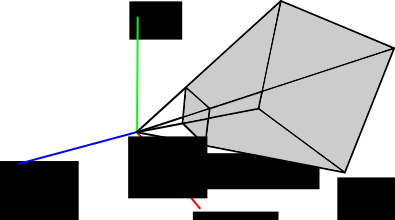
\includegraphics{view_frustum.pdf}
	\caption{The view frustum for perspective camera model.}
	\label{figure:view_frustum}
\end{figure}

There are two concepts associated with the camera. The first one is orientation in 3-dimensional space. To define the orientation a position and three normalized vectors, mutually perpendicular, must be specified. That triple forms the orthogonal basis. In figure \ref{figure:view_frustum} there are three such vectors which form the right-handed coordinate system (since $R \times U = F$, where $\times$ denotes the cross product) with the eye point $E$.

Given a point $P$ in "global" Cartesian space we can easily find its coordinates $P'$ in so-called \textbf{camera space} (or \textbf{view space}). In \textbf{camera space} $E$ is the origin, and the triple $R$, $U$ and $F$ serve as the cardinal axes $X$, $Y$ and $Z$. Position of $P$ in Cartesian space, but being defined in terms of \textbf{camera space} (\cite{eberly}), is:
\begin{equation}
	\label{equation:camera_space}
	P = E + rR + uU + fF
\end{equation}
Assuming $R$, $U$ and $F$ form the orthogonal basis, the position of point $P$ in \textbf{camera space} is $P' = (r, u, f)$. So the problem now is to determine $r$, $u$ and $f$ from equation \ref{equation:camera_space}. Let us compute $r$:
\begin{eqnarray*}
	P &=& E + rR + uU + fF \\[0.3em]
	rR &=& P - E - uU - fF \\[0.3em]
	rR \cdot R &=& (P - E) \cdot R - uU \cdot R - fF \cdot R \\[0.3em]
	r &=& (P - E) \cdot R
\end{eqnarray*}
In the calculations above we utilized the facts: $R \cdot R = 1$, $R \cdot U = 0$ and $R \cdot F = 0$ (where $\cdot$ symbol denotes the dot product). Calculations of $u$ and $f$ are analogous.

The second concept related to the view frustum is the area that will be visible to the viewer. In figure \ref{figure:view_frustum} it is marked with the grey region. To define that area, six values are used:
\begin{itemize}
	\item distance $n$ from the origin $E$ to a so-called near plane (nothing in front of this plane will be rendered);
	\item distance $f$ from the origin $E$ to a so-called far plane (nothing behind this plane will be rendered);
	\item width of the near plane (which is controlled by two values, one defining bound in the $-R$ direction, and one defining bound in the $+R$ direction);
	\item height of the near plane (which is controlled by two values, one defining bound in the $-U$ direction, and one defining bound in the $+U$ direction).
\end{itemize}

To render the 3-dimensional world on the 2-dimensional screen we must take all the geometry that is visible in the grey region and then project it to the near plane. The section \ref{subsubsection:vertex_transformation} discusses in details the whole process.

\subsection{Vertex Processing}

Vertex processing is the first of the two (the second is pixel processing) general stages that the input virtual world goes through. The vertex processor has three main goals:
\begin{itemize}
	\item transformation of vertices from the 3-dimensional representation to the 2-dimensional one;
	\item rejection from the pipeline of triangles that are not visible to the viewer (like those residing outside the view frustum);
	\item clipping of triangles that intersect the near plane of the view frustum.
\end{itemize}
All of these aspects are investigated in details in the following sections.

\subsubsection{Vertex Transformation}
\label{subsubsection:vertex_transformation}

Objects in the virtual world are made with triangles. Computer graphics artists usually use specialized software, like Blender or 3D Studio Max, to create these objects. The artist usually creates their object in some local coordinate space of the graphics program. We can imagine an object being created with triangles, "standing" in the $XZ$ plane, where $Y = 0$, somewhere around the origin point $O = (0, 0, 0)$. An example is depicted in figure \ref{figure:modelling_object_in_blender}.
\begin{figure}
	\centering
	\includegraphics[scale=0.35]{modelling_object_in_blender.png}
	\caption{An object being modelled in Blender.}
	\label{figure:modelling_object_in_blender}
\end{figure}

Now let's assume that this object has been loaded to the application, and we want it to be rendered at position $P = (3, 0, 5)$. We keep in mind, that the object has been modelled in its local coordinate space, at the origin point $O$. So if we want to render the object at the position $P$, before rendering, we need to transform this object. In this case transformation is simply a translation by a vector.

Given the input set of vertices $\mathcal{IV}$ that define the object (namely, the triangles of the object), we want to produce the output set of vertices\footnote{Note that at this moment by referring to vertices, we actually refer to their positions, omitting colors and texture coordinates for the sake of argument.} $\mathcal{OV}$, translated by the point $P$ (vertices are indexed with $i$):
	$$ \mathcal{OV}_i = \mathcal{IV}_i + P = \mathcal{IV}_i + (3, 0, 5) $$
The transformation that has just been carried out moves the object from so-called \textbf{object space} (or \textbf{model space}) to so-called \textbf{world space}. Thus the name of the transformation is world transformation.

One might wonder why bother with local coordinates if we could have set the object in point $P$ directly in the modelling program and import the already-transformed object. This is indeed true, but \textbf{object space} has some very important feature --- instancing. What if we were to put five instances of the object in various places? We would have to store five times more geometry for the same one object. By having the object in the local coordinates (usually near the origin $O = (0, 0, 0)$) we can reuse its geometry many times, using different translation vectors (storing a pointer to an object and a translation vector takes much less memory than storing the object itself). Of course, the number of generated output vertices will be the same, but we have at least saved memory for the input set.

Direct translation by a vector is one form of altering positions of vertices. However, a much neater and compact way is to use $4 \times 4$ matrices:
\[
	\begin{bmatrix}
		x' & y' & z' & w'
	\end{bmatrix}
	=
	\begin{bmatrix}
		x & y & z & 1
	\end{bmatrix}
	\begin{bmatrix}
		1 & 0 & 0 & 0 \cr
		0 & 1 & 0 & 0 \cr
		0 & 0 & 1 & 0 \cr
		t_x & t_y & t_z & 1
	\end{bmatrix}
	=
	\begin{bmatrix}
		x + t_x & y + t_y & z + t_z & 1
	\end{bmatrix}
\]
To form a $4 \times 4$ translation matrix, it is enough to just put the translation vector in the last row (this is row-major order) to the indentity matrix.

The matrix form of vector translation depicted above exhibits a very important concept --- homogenous coordinates. Homogenous coordinates are a way of transforming a 3-dimensional vertex through a $4 \times 4$ matrix. Since the vertex has three coordinates, it cannot be multiplied by the matrix. A solution is to extend the triple $(x, y, z)$ to the quadruple of general form $(x, y, z, w)$. This way we actually move from the 3rd to the 4th dimension. Of course, the additional dimension is rather dummy and we set a fixed value of $1$ to the $w$-coordinate. Note that after the transformation we end up with a vector that also satisfies $w = 1$, what means that the output vector $(x', y', z')$ is in the same 3-dimensional space as the input vector $(x, y, z)$. The extension with $w$-coordinate had only one purpose --- it allowed us to put a vector translation to a matrix.

A question that can arise now is whether the output vector's $w$-coordinate is different than $1$. The $w$-coordinate will be different than $1$ if and only if the 4th column of the matrix (through which the input vector is multiplied by) is different than $[0\ 0\ 0\ 1]^\mathrm{T}$. Translation matrix has the 4th column in that form so the resulting $w$-coordinate is guaranteed to be $1$ (if the input $w$-coordinate is $1$). In case when it is not (like in perspective projection matrix that will be discussed later in this chapter), a projection must be applied such that the $w$-component is equal to $1$. It can be achieved by simply dividing all components of the output vector by the $w$-component:
\[
	\begin{bmatrix}
		x & y & z & w
	\end{bmatrix}
	\sim
	\begin{bmatrix}
		\frac{x}{w} & \frac{y}{w} & \frac{z}{w} & \frac{w}{w}
	\end{bmatrix}
	=
	\begin{bmatrix}
		\frac{x}{w} & \frac{y}{w} & \frac{z}{w} & 1
	\end{bmatrix}
\]
Note the $\sim$ symbol, which denotes "is equivalent to". A vertex before a so-called perspective division is said to be in \textbf{homogenous clip space}. After the perspective division it holds almost the same information (from a geometrical point of view) as the input one, missing only the $w$-component. The output vertex is a 3-dimensional representation of the 4-dimensional input vertex.

To shortly sum up why we use $4 \times 4$ matrices in computer graphics is the fact that they can represent linear, affine and perspective transformations altogether within one single matrix. Since a whole lot of matrices (translation, rotation, reflection, projection) can be represented with $4 \times 4$ matrices, and moreover all transformations can be combined via matrix multiplication in a single matrix, it is possible to derive one $4 \times 4$ matrix which, based on the virtual camera parameters, can transform a 3-dimensional vertex to its 2-dimensional position on the screen (namely, on the view frustum's near plane). The derivation process of such one matrix is discussed throughout this section.

Once the objects have been transformed to global \textbf{world space}, it comes the time to utilize the virtual camera we discussed in section \ref{subsubsection:virtual_camera}. We do so by transforming all vertices from \textbf{world space} to \textbf{view space} via view transformation matrix. The goal of this matrix is simply to get world positions of the vertices with respect to the camera's position and orientation. We already know that we can compute a vertex's position (given in "global" Cartesian space, and this space in this case is our \textbf{world space}) with respect to a camera via equation \ref{equation:camera_space}. The final coordinates $P' = (r, u, f)$ in \textbf{camera space} of a vertex $P = (x, y, z)$ given in \textbf{world space} are:
\begin{eqnarray*}
	r &=& (P - E) \cdot R \\[0.3em]
	u &=& (P - E) \cdot U \\[0.3em]
	f &=& (P - E) \cdot F
\end{eqnarray*}
This transformation can be represented in a nice matrix form:
\[
	\begin{bmatrix}
		r & u & f & 1
	\end{bmatrix}
	=
	\begin{bmatrix}
		x & y & z & 1
	\end{bmatrix}
	\begin{bmatrix}
		1 & 0 & 0 & 0 \cr
		0 & 1 & 0 & 0 \cr
		0 & 0 & 1 & 0 \cr
		-E_x & -E_y & -E_z & 1
	\end{bmatrix}
	\begin{bmatrix}
		R_x & U_x & F_x & 0 \cr
		R_y & U_y & F_y & 0 \cr
		R_z & U_z & F_z & 0 \cr
		0 & 0 & 0 & 1
	\end{bmatrix}
\]

It is said that a picture is worth more than a thousand words. Figure \ref{figure:view_transform} presents what this transformation actually does.
\begin{figure}
	\centering
	\subfloat[The box and the camera in \textbf{world space}.]
	{
		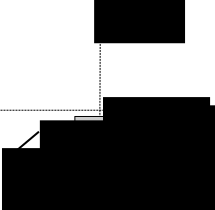
\includegraphics{view_transform_a.pdf}
	}
	\subfloat[The box after transformation to \textbf{view space}.]
	{
		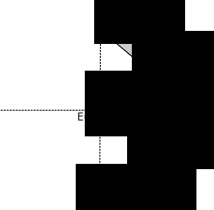
\includegraphics{view_transform_b.pdf}
	}
	\caption{A box and a camera in different spaces.}
	\label{figure:view_transform}
\end{figure}
As can be seen (a top-down view along the $Y$-axis), the view transformation simply moves (and rotates) objects in such a way, as if the camera was placed in the origin, having its basis vectors aligned with the cardinal axes $X$, $Y$ and $Z$ of the world. Note that in \textbf{view space} the $z$-coordinate (or rather its absolute value) of a vertex is at the same time its distance to the camera. This will be very important in determining which cover mutually, so that we can draw them in correct order.

It is worth noting that the introduction of \textbf{view space} in a way we introduced it is not mandatory. However, it makes further processing of geometry (projection mostly) much easier and thus performing this step is very popular.

After the objects have went through the world and view transformations, they can be projected on the near plane of the view frustum. Projection is a relatively easy concept --- we want the objects that are farther from the camera to appear smaller on the near plane than the objects that are closer.

Let us examine a simple case of projection a point onto the near plane (our considerations will take place in the $YZ$ plane for simplicity), shown in figure \ref{figure:projection}.
\begin{figure}
	\centering
	
\includegraphics{projection.pdf}
	\caption{Projection of a point onto the near plane.}
	\label{figure:projection}
\end{figure}
To find the projected point (of point $(y, z)$) on the near plane\footnote{Note that both the near and far planes have negative signs. This is correct because the input values $n$ and $f$ define the distances from the planes (which are always positive). Here, we mark the coordinates, and since we are working in a right-handed coordinate system, with the camera looking down the negative $Z$-axis, the $z$-coordinates of the planes are $-n$ and $-f$.} at position $(y', -n)$, we simply use Thales theorem which in this case states that:
\begin{eqnarray*}
	\frac{-n}{y'} &=& \frac{z}{y} \\[0.3em]
	y' &=& \frac{-ny}{z}
\end{eqnarray*}
The value of $x'$ can be analogously computed as:
	$$ x' = \frac{-nx}{z} $$
Let us see how to encompass these equations in a matrix:
\[
	\begin{bmatrix}
		x & y & z & 1
	\end{bmatrix}
	\begin{bmatrix}
		-n & 0 & 0 & 0 \cr
		0 & -n & 0 & 0 \cr
		0 & 0 & A & 1 \cr
		0 & 0 & B & 0
	\end{bmatrix}
	=
	\begin{bmatrix}
		-nx & -ny & Az + B & z
	\end{bmatrix}
	\sim
	\begin{bmatrix}
		-\frac{nx}{z} & -\frac{ny}{z} & A + \frac{B}{z} & 1
	\end{bmatrix}
\]
It is obvious that a division cannot be included in a matrix operation. That is why we employ the $w$-coordinate here, in which we must put the input $z$-coordinate. This way we get the output vertex with $w' = z$, and we can use the perspective division to obtain the final point.

It was quite easy to handle the $x$- and $y$- coordinates. A problem that remains is transformation of $z$. Quick considerations lead us to a conclusion, that we do not want the $z$-coordinate to be transformed at all, we just want to pass it as is through the matrix. So we must find suitable coefficients in the 3rd column of the perspective matrix. The first two we know are zeroes, what means that the output $z$-coordinate will not be dependent on the input $x$- and $y$- coordinates. We put $A$ and $B$ later on what indicates that $z'$ will have a form of linear mapping (after the perspective division):
\begin{equation}
	\label{equation:z_mapping}
	F(z) = A + \frac{B}{z} 
\end{equation}
If we just want the $z$ to be passed as is, we need to map the range $[-n, -f]$ to the range $[-n, -f$]. This way we can solve equation \ref{equation:z_mapping} for $A$ and $B$ with the following constraints:
	$$ F(-n) = A + \frac{B}{-n} = -n $$
	$$ F(-f) = A + \frac{B}{-f} = -f $$
Straight algebra manipulations lead to:
\begin{eqnarray*}
	A &=& -(n + f) \\[0.3em]
	B &=& -nf
\end{eqnarray*}
The final perspective projection matrix is:
\[
	\begin{bmatrix}
		-n & 0 & 0 & 0 \cr
		0 & -n & 0 & 0 \cr
		0 & 0 & -(n + f) & 1 \cr
		0 & 0 & -nf & 0
	\end{bmatrix}
\]
Note that despite the output $z$-coordinate satisfies $F(-n) = -n$ and $F(-f) = -f$, it does not satisfy $F(z) = z$ for $z$ in the range $(-n, -f)$. In fact, $z$-coordinates change with respect to $\frac{1}{z}$ curve, as equation \ref{equation:z_mapping} states.

The perspective projection matrix that has just been derived is fully correct, but has one flaw --- it reflects the coordinates in \textbf{homogenous clip space}. The input $x$ becomes $-nx$, for instance. We can avoid this artifact by multiplying all coordinates by $-1$ before the matrix multiplication. This is fully allowed operation because the output vertex position after the perspective division will remain unchanged:
\[
	k
	\begin{bmatrix}
		x & y & z & 1
	\end{bmatrix}
	=
	\begin{bmatrix}
		kx & ky & kz & k
	\end{bmatrix}
	\sim
	\begin{bmatrix}
		\frac{kx}{k} & \frac{ky}{k} & \frac{kz}{k} & \frac{k}{k}
	\end{bmatrix}
	=
	\begin{bmatrix}
		x & y & z & 1
	\end{bmatrix}
\]
The multiplication by $-1$ effect is achieved simply by multiplying by $-1$ all entries of the perspective matrix:
\[
	\begin{bmatrix}
		x & y & z & 1
	\end{bmatrix}
	\begin{bmatrix}
		n & 0 & 0 & 0 \cr
		0 & n & 0 & 0 \cr
		0 & 0 & -A & -1 \cr
		0 & 0 & -B & 0
	\end{bmatrix}
	=
	\begin{bmatrix}
		nx & ny & -Az - B & -z
	\end{bmatrix}
	\sim
	\begin{bmatrix}
		-\frac{nx}{z} & -\frac{ny}{z} & A + \frac{B}{z} & 1
	\end{bmatrix}
\]
As can be noticed, the output vertex, after the perspective division, has not changed.

At this moment all vertices have their positions on the near plane of the virtual camera. The next step is to introducte orthogonal transformation, which will map all visible points (on the near plane) to the normalized $[-1, 1] \times [-1, 1] \times [-1, 1]$ unit cube. We want all vertices that lie within that cube to be visible to the camera.

We start with the four parameters of the virtual camera, which specify the camera near plane's left ($l$), right ($r$), bottom ($b$) and top ($t$) bounds. We want the following linear mappings:
\begin{eqnarray*}
	-1 &=& a_x l + b_x \\[0.3em]
	1 &=& a_x r + b_x
\end{eqnarray*}
\begin{eqnarray*}
	-1 &=& a_y b + b_y \\[0.3em]
	1 &=& a_y t + b_y
\end{eqnarray*}
\begin{eqnarray*}
	-1 &=& a_z (-n) + b_z \\[0.3em]
	1 &=& a_z (-f) + b_z
\end{eqnarray*}
Solving them yields:
\begin{eqnarray*}
	a_x &=& \frac{2}{r - l} \\[0.3em]
	b_x &=& -\frac{r + l}{r - l}
\end{eqnarray*}
\begin{eqnarray*}
	a_y &=& \frac{2}{t - b} \\[0.3em]
	b_y &=& -\frac{t + b}{t - b}
\end{eqnarray*}
\begin{eqnarray*}
	a_z &=& -\frac{2}{f - n} \\[0.3em]
	b_z &=& -\frac{n + f}{f - n}
\end{eqnarray*}
Written in matrix form:
\[
	\begin{bmatrix}
		\frac{2}{r - l} & 0 & 0 & 0 \\[0.3em]
		0 &  \frac{2}{t - b} & 0 & 0 \\[0.3em]
		0 & 0 & -\frac{2}{f - n} & 0 \\[0.3em]
		-\frac{r + l}{r - l} & -\frac{t + b}{t - b} & -\frac{n + f}{f - n} & 1
	\end{bmatrix}
\]

After transformation of a vertex $P = (x, y, z, 1)$ through the world, view, perspective and orthogonal matrices (but before the perspective divide!), the vertex will receive a new position $P' = (x', y', z', w')$ in \textbf{homogenous clip space}, where determining whether a point is visible to the camera can be achieved by checking the following constraints:
	$$ -w' \le x' \le w' $$
	$$ -w' \le y' \le w' $$
	$$ -w' \le z' \le w' $$
After dividing by $w'$ and receiving $P'' = (x'', y'', z'', 1)$, the constraints turn into the desired unit cube:
	$$ -1 \le x'' \le 1 $$
	$$ -1 \le y'' \le 1 $$
	$$ -1 \le z'' \le 1 $$

The final step is to map the unit cube to the screen. Let us say we have a screen sized $width \times height$. We want to perform yet another linear mapping that will take the $XY$ unit square of the unit cube to the rectangle $[0, width] \times [0, height]$.

The transformation matrix to \textbf{window space}:
\[
	\begin{bmatrix}
		\frac{width}{2} & 0 & 0 & 0 \\[0.3em]
		0 & \frac{height}{2} & 0 & 0 \\[0.3em]
		0 & 0 & 1 & 0 \\[0.3em]
		\frac{width}{2} & \frac{height}{2} & 0 & 1
	\end{bmatrix}
\]

One mind wonder why orthogonal and window transformations have not been carried out together, since they both represent some sort of linear mappings. The reason is simply convenience. It is sometimes very intuitive to introduce a sort of "normalization" (what orthogonal projection does).

Let us now remind all the matrices that an input vertex $P = (x, y, z, 1)$ must be passed through to finally appear on the screen:
\[
	\textbf{World} =
	\begin{bmatrix}
		m_{11} & m_{12} & m_{13} & m_{14} \cr
		m_{21} & m_{22} & m_{23} & m_{24} \cr
		m_{31} & m_{32} & m_{33} & m_{34} \cr
		m_{41} & m_{42} & m_{43} & m_{44}
	\end{bmatrix}
\]
\[
	\textbf{View} =
	\begin{bmatrix}
		1 & 0 & 0 & 0 \cr
		0 & 1 & 0 & 0 \cr
		0 & 0 & 1 & 0 \cr
		-E_x & -E_y & -E_z & 1
	\end{bmatrix}
	\begin{bmatrix}
		R_x & U_x & F_x & 0 \cr
		R_y & U_y & F_y & 0 \cr
		R_z & U_z & F_z & 0 \cr
		0 & 0 & 0 & 1
	\end{bmatrix}
\]
\[
	\textbf{Perspective} =
	\begin{bmatrix}
		n & 0 & 0 & 0 \cr
		0 & n & 0 & 0 \cr
		0 & 0 & n + f & -1 \cr
		0 & 0 & nf & 0
	\end{bmatrix}
\]
\[
	\textbf{Orthogonal} =
	\begin{bmatrix}
		\frac{2}{r - l} & 0 & 0 & 0 \\[0.3em]
		0 &  \frac{2}{t - b} & 0 & 0 \\[0.3em]
		0 & 0 & -\frac{2}{f - n} & 0 \\[0.3em]
		-\frac{r + l}{r - l} & -\frac{t + b}{t - b} & -\frac{n + f}{f - n} & 1
	\end{bmatrix}
\]
\[
	\textbf{Window} =
	\begin{bmatrix}
		\frac{width}{2} & 0 & 0 & 0 \\[0.3em]
		0 & \frac{height}{2} & 0 & 0 \\[0.3em]
		0 & 0 & 1 & 0 \\[0.3em]
		\frac{width - 1}{2} & \frac{height - 1}{2} & 0 & 1
	\end{bmatrix}
\]
\begin{eqnarray*}
	P' &=& P * \textbf{World} * \textbf{View} * \textbf{Perspective} * \textbf{Orthogonal} * \textbf{Window} \\[0.3em]
	P'' &=& ( \frac{P'_x}{P'_w}, \frac{P'_y}{P'_w}, \frac{P'_z}{P'_w}, 1 )
\end{eqnarray*}
The values $P''_x$ and $P''_y$ represent the vertex $P$'s position on the screen (\textbf{screen space}), and the value $P''_z$ represents a scaled, non-uniformly distorted (due to perspective projection) distance of the vertex to the camera, which is in the range $[-1, 1]$ ($-1$ means the vertex $P$ lies on the near plane, $1$ means the vertex $P$ lies on the far plane).

Vainmoinen provides helper functions \texttt{constructViewTransform} for constructing $\textbf{View}$ matrix and \texttt{constructProjTransform} for constructing combined $\textbf{Perspective} * \textbf{Orthogonal}$ matrix. The user does not have to take care of window transform, as this is applied by Vainmoinen internally.

\subsubsection{Triangle Culling}

Some triangles can be culled (rejected from further processing). There are two types of culling: view frustum culling and backface culling. The former one is responsible for rejecting triangles that are not visible in the view frustum --- they do not have to be rasterized on the screen as they are simply not visible. The latter, backface culling, rejects triangles that face away from the camera. Introduction of a concept of a face of a triangle helps to eliminate around one half of visible triangles, that would not be seen anyway.

View frustum culling can be performed in \textbf{world space}. To do so, we must find equations of the view frustum planes, and check each triangle against these planes. Figure \ref{figure:view_frustum_culling} depicts an example situation where triangles are to be tested for visibility against the view frustum (a top-down view).
\begin{figure}
	\centering
	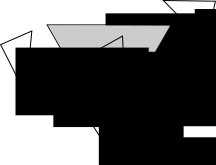
\includegraphics{view_frustum_culling.pdf}
	\caption{View frustum culling.}
	\label{figure:view_frustum_culling}
\end{figure}

Assuming the equations of the planes are known, the simplest algorithm for determining whether a triangle is outside the view frustum is to check whether all its vertices are on one side of a plane. For example, it is clear that triangle $1$ is outside the view frustum, since all of its vertices lie on the outer side of the left plane (we assume that the planes' normal vectors are directed to the view frustum). The same is true for triangle $2$, which lies on the outer side of the near plane.

The triangles marked as $3$ and $4$ will both be rendererd. The first one lies on the inner sides of all planes so it is obviously visible. Triangle $4$ intersects the right plane and thus is also visible (it does not lie on the outer side of any plane).

The most interesting case is classification of triangle $5$. Obviously, it is not visible in the view frustum, yet it will not be rejected. The problem is that the triangle intersects the right and top planes and hence does not lie on the outer side of either of them. At first it might seem to be a big problem, but in practice it is meaningless. The triangle lies outside the view frustum and although it will be passed to the rasterizer, even one processor's cycle will be wasted for its rendering (only a few computations and memory will get wasted for some other type of processing on a per-triangle basis).

Our considerations were related to \textbf{world space}. Of course, nothing prevents us from doing the visibility tests in \textbf{view space} or even in \textbf{homogenous clip space} (before the perspective divide). That is where Vainmoinen (OpenGL and Direct3D also) does view frustum culling. It has a few advantages. Firstly, the view frustum planes have much neater representation in that space (since the view frustum is a cube). Secondly, the renderer does not need to store the planes' equations nor even compute them. All it expects is the combined $\textbf{World} * \textbf{View} * \textbf{Perspective} * \textbf{Orthogonal}$ matrix, then the renderer does view frustum culling, perspective divide, and finally transforms the visible vertices by the \textbf{Window} matrix.

The planes' equations (in \textbf{homogenous clip space}) are:
\begin{eqnarray*}
	left:\ \ \ x + w &=& 0 \\[0.3em]
	right:\ \ \  x - w &=& 0 \\[0.3em]
	bottom:\ \ \ y + w &=& 0 \\[0.3em]
	top:\ \ \ y - w &=& 0 \\[0.3em]
	near:\ \ \ z + w &=& 0 \\[0.3em]
	far:\ \ \ z - w &=& 0 
\end{eqnarray*}
Note that these are 4-dimensional hyperplanes. The left plane, for instance, has a 4-dimensional normal vector $[1\ 0\ 0\ 1]$ and is away by $0$ units from the origin $(0, 0, 0, 0)$.

The second type of culling is backface culling. The idea is to cull triangles  that face away from the camera. To do so, we must first introduce a concept of a side of a triangle to know whether it is considered front or back facing. This is related to order in which vertices of a triangle are specified. Figure \ref{figure:vertices_ordering} presents the two types of ordering that can be applied to a triangle: counter-clockwise (CCW) and clockwise (CW).
\begin{figure}
	\centering
	\subfloat[Counter-clockwise (CCW) ordering.]
	{
		
\includegraphics{vertices_ordering_ccw.pdf}
	}
	\hspace{40pt}
	\subfloat[Clockwise (CW) ordering.]
	{
		
\includegraphics{vertices_ordering_cw.pdf}
	}
	\caption{Counter-clockwise (CCW) and clockwise (CW) vertices ordering.}
	\label{figure:vertices_ordering}
\end{figure}

To detect what type of ordering has been applied to a triangle, the cross product can be used. Let us form two vectors from the vertices, $v_1v_0$ and $v_2v_0$. The resulting vector is perpendicular to both, and will point out of this page if the ordering is CCW, or will point into this page if the ordering is CW.

The goal of backface culling is to reject either all triangles that have CCW ordering or CW ordering. The test is performed in \textbf{window space}, after projection of the triangles onto the screen.

One might wonder why to actually reject triangles with respect to their facing. The motivation is that most objects that we deal with in virtual worlds are, from mathematical standpoint, 2-manifolds, what simply means that the objects are closed volumes, where each edge is shared by exactly two triangles. With backface culling we can reject from the pipeline the triangles that are not visible to the camera (because they are inner triangles that are covered by outer triangles).

Let us consider a cube (which is a 2-manifold object) as depicted in figure \ref{figure:cube}.
\begin{figure}
	\centering
	
\includegraphics{cube.pdf}
	\caption{A cube with numbered vertices.}
	\label{figure:cube}
\end{figure}
For the sake of argument let us deal with quads instead of triangles. The cube in figure \ref{figure:cube} can be described with six quads: $front = 0123$, $left = 7610$, $back = 4567$, $right = 3254$, $top = 7034$ and $bottom = 1652$. Note that all these quads have CCW ordering in \textbf{world space} --- imagine standing in front of each quad and following the indices of vertices of each quad's definition. However, after projecting the vertices onto the screen plane, the ordering of some quads changes. The ordering of quads $front$, $right$ and $top$ is still CCW, but the ordering of $left$, $back$ and $bottom$ switches to CW. Since the cube is a 2-manifold, we can safely reject $left$, $back$ and $bottom$ quads, as they are fully covered by $front$, $right$ and $top$ quads. This will be true for any set of CCW-ordered and CW-ordered triangles. In general, if triangle's vertices in \textbf{world space} are given in some fixed (CCW or CW) order, and this order switches after transformation to \textbf{screen space}, then the triangle is certainly covered by another triangle (in case when the triangle is part of a 2-manifold object) and can be rejected.

Vainmoinen expects the triangles to be passed in CCW order and will reject all those whose ordering switches to CW after projection to \textbf{screen space}.

\subsubsection{Triangle Clipping}

There is one more step that must be applied to triangles before passing them to the pixel processor. This step is triangle clipping. The triangles must be clipped to the near plane, and optionally can be clipped to the other planes of the view frustum.

Let us take a look at figure \ref{figure:clipping}.
\begin{figure}
	\centering
	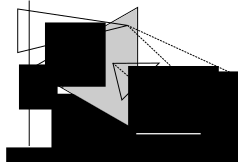
\includegraphics{clipping.pdf}
	\caption{Triangle clipping to the near and far planes.}
	\label{figure:clipping}
\end{figure}
Triangle $1$ intersects the far plane so only part of it is visible in the view frustum. If so, then we would like to cut off the part that is not visible, so that it does not get rendered by the pixel processor. We can clip the triangle to the far plane and reject the outside part. Note however, that the remaining part of the triangle has turned into a polygon with four vertices. To be able to process it, we must first split that polygon in two triangles, as a dashed line indicates.

The fact is that clipping to the far plane is not mandatory. We could have left triangle $1$ untouched and pass it to the rasterizer. The rasterizer could detect parts of the triangle that are outside of the view frustum simply by checking $z$-coordinates of pixels of the triangle. Those pixels that satisfy $z > 1$ are not visible.

Clipping can also be avoided with repsect to the left, right, bottom and top planes. The reasoning is the same as with the far plane. Given vertices' coordinates on the screen, that is, in square $[0, width - 1] \times [0, height - 1]$, we can quickly reject the pixels that are outside the view frustum.

As has been stated at the beginning of this section, clipping to the near plane must be done. Let us take a look at figure \ref{figure:clipping} again. Triangle $2$ intersects the near plane. So what is wrong with it and why does it have to be clipped? Well, in fact this triangle does not have to. It can be passed to the rasterizer as well as triangle $1$ was, and to avoid drawing the part that is invisible, we would have to make additional test $z < -1$. However, the problem arises in case of triangle $3$. The problem with it is that it intersects the eye plane. The perspective projection matrix has the effect of "mirroring" vertices that lie behind the eye $E$. So after multiplying the vertex by a whole chain of matrices discussed in section \ref{subsubsection:vertex_transformation}, and after (this is crucial here) dividing the result by $w$-coordinate, the vertices that are behing the eye, will end up somewhere behind the far plane. This means that if we do not apply clipping to triangle $3$, the triangle that will get to the rasterizer will be triangle $3'$. Actually, the plane to which the triangles must be clipped does not have to be the near plane. It can be any plane "between" the eye and near plane, but if one chooses such option then they must remember about the condition $z \ge -1$ in the rasterizer. If we clip to the near plane (what Vainmoinen does), then this test is redundant.

We already know we have to clip to the near plane. We can do so in any space but, what is crucial, it has to be done before the perspective $w$-division. Clipping can be done in \textbf{world space} (what is the most intuitive solution) but Vainmoinen, as well as OpenGL and Direct3D, does so (as well as triangle culling) in 4-dimensional \textbf{homogenous clip space}. This is very interesting situation because clipping of 4-dimensional triangles takes place here, with a 4-dimensional hyperplane passing through the origin $(0, 0, 0, 0)$. This shows the beauty of mathematics --- we do totally unintuitivie computations and obtain (after the perspection division) totally intuitive results.

Let us now get to the heart of the problem, namely, how to find an intersection point of a line (triangle's edge) with a plane. The implicit plane equation in vector form is:
	$$ N \cdot (P - P_0) = 0 $$
Since we know that the near plane (which is a hyperplane in \textbf{homogenous clip space}) is passing through the origin $(0, 0, 0, 0)$, we can thus write:
\begin{equation}
	\label{equation:plane_equation}
	N \cdot P = 0
\end{equation}
The explicit parametric line equation is:
\begin{equation}
	\label{equation:line_equation}
	P = P_0 + tV
\end{equation}
To find the intersection point we simply plug equation \ref{equation:line_equation} into equation \ref{equation:plane_equation}:
	$$ N \cdot (P_0 + tV) = 0 $$
	$$ t = -\frac{N \cdot P_0}{N \cdot V} $$
The normal vector $N$ for the 4-dimensional near plane is either $-[0\ 0\ 1\ 1]$ or $[0\ 0\ 1\ 1]$.

\subsection{Pixel Processing}

When a triangle successfully gets out of the vertex processor it goes to the pixel processor, which draws the triangle on the screen. This section discusses details of how this process is being proceed.

\subsubsection{Rasterization and Shading}
\label{subsubsection:rasterization_and_shading}

The goal of rasterization is to find all pixels that belong to a triangle, compute pixels' attributes (like color and texture coordinate) and finally shade the pixels. Attributes are computed by interpolating values that come from the vertices of the triangle. Shading process uses this interpolated values to produce the final colors of the pixels.

Finding pixels of a triangle is not a trivial task. The most naive method is to loop through all pixels of the screen, and check each pixel if it belongs to the triangle. If it does, then attributes of the pixel are computed; if it does not, the loop goes to the next pixel. This method is very ineffective since a triangle can cover a very small portion of the screen, yet all screen's pixels must be processed to rasterize it.

To strongly alleviate the processing power needed to process a single triangle, a very simple approach can by utilized. The idea is to find a triangle's bounding box in \textbf{screen space}, and process only pixels that lie within that box. Figure \ref{figure:bounding_box} depicts a triangle and its bounding box.
\begin{figure}
	\centering
	
\includegraphics{bounding_box.pdf}
	\caption{A triangle and its bounding box.}
	\label{figure:bounding_box}
\end{figure}

Let us assume a triangle has \textbf{screen space} vertices $v_0 = (x_0, y_0)$, $v_1 = (x_1, y_1)$ and $v_2 = (x_2, y_2)$, and the screen has resolution $width \times height$. A bounding box for this triangle is defined as:
\begin{eqnarray*}
	\mbox{min3}(a, b, c) &=& \mbox{min}(a, \mbox{min}(b, c)) \\[0.3em]
	\mbox{max3}(a, b, c) &=& \mbox{max}(a, \mbox{max}(b, c))
\end{eqnarray*}
\begin{eqnarray*}
	min_x &=& \mbox{max}(\mbox{min3}(x_0, x_1, x_2), 0) \\[0.3em]
	max_x &=& \mbox{min}(\mbox{max3}(x_0, x_1, x_2), width - 1)
\end{eqnarray*}
\begin{eqnarray*}
	min_y &=& \mbox{max}(\mbox{min3}(y_0, y_1, y_2), 0) \\[0.3em]
	max_y &=& \mbox{min}(\mbox{max3}(y_0, y_1, y_2), height - 1)
\end{eqnarray*}
Having such defined bounding box we can now process the area $[min_x, min_y] \times [max_x, max_y]$ of pixels, rather than $[0, 0] \times [width - 1, height - 1]$.

Altough we have greatly reduced the number of pixels that are to be processed, we still do not know which of them belong to the triangle. To solve this issue we will employ so-called barycentric coordinates (based on discussion in \cite{shirley}), that will not only help us to decide whether a pixel belongs to the triangle or not, but will almost automatically perform interpolation of attributes.

An arbitrary vertex on a triangle's plane can be represented as a weighted average of its vertices:
\begin{equation}
	\label{equation:barycentric_coordinates_1}
	v = \alpha * v_0 + \beta * v_1 + \gamma * v_2
\end{equation}
By adding to equation \ref{equation:barycentric_coordinates_1} the following constraint:
\begin{equation}
	\label{equation:barycentric_coordinates_constraint}
	\alpha + \beta + \gamma = 1
\end{equation}
the triple $[\alpha, \beta, \gamma]$ is reffered to as barycentric coordinates. Constraint \ref{equation:barycentric_coordinates_constraint} has a very nice property that guarantees that barycentric coordinates of a point on the triangle's plane, that belongs to the triangle (excluding its edges), satisfy the following inequalities:
\begin{eqnarray*}
	0 < \alpha < 1 \\[0.3em]
	0 < \beta < 1 \\[0.3em]
	0 < \gamma < 1
\end{eqnarray*}
On the other hand, if the point belongs to the triangle, including its edges, then the inequalities turn into:
\begin{eqnarray*}
	0 \le \alpha \le 1 \\[0.3em]
	0 \le \beta \le 1 \\[0.3em]
	0 \le \gamma \le 1
\end{eqnarray*}

Equation \ref{equation:barycentric_coordinates_1} can be easily generalized to any attribute $u$ (like color or texture coordinate):
	$$ u = \alpha * u_0 + \beta * u_1 + \gamma * u_2 $$

Let us consider signed distances marked in figure \ref{figure:barycentric_coordinates}.
\begin{figure}
	\centering
	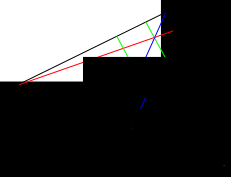
\includegraphics{barycentric_coordinates.pdf}
	\caption{Distances marked for barycentric coordinates computation.}
	\label{figure:barycentric_coordinates}
\end{figure}
To compute barycentric coordinates of point $P$, we use the following formulas:
\begin{eqnarray*}
	\alpha = \frac{a_2}{a_1} \\[0.3em]
	\beta = \frac{b_2}{b_1} \\[0.3em]
	\gamma = \frac{c_2}{c_1}
\end{eqnarray*}

The pseudocode in listing \ref{listing:rasterization_1} shows how to rasterize a triangle on the screen by interpolating color values from its vertices.
\begin{lstlisting}[label=listing:rasterization_1, caption={Rasterization of a triangle.}]
a1 = distance(v0.position.xy, line_v1v2)
b1 = distance(v1.position.xy, line_v2v0)
c1 = distance(v2.position.xy, line_v0v1)

for y = minY to maxY
	for x = minX to maxX

		a2 = distance((x, y), line_v1v2)
		b2 = distance((x, y), line_v2v0)
		c2 = distance((x, y), line_v0v1)

		alpha = a2 / a1
		beta = b2 / b1
		gamma = c2 / c1

		if (alpha >= 0 and beta >= 0 and gamma >= 0)
			colorBuffer(x, y) = alpha*v0.color + beta*v1.color + gamma*v2.color
\end{lstlisting}

In line 16 we check whether the coordinates are all greater than or equal to $0$. Theoretically, we should also check whether these coordinates are smaller than or equal to $1$. However, from the constraint \ref{equation:barycentric_coordinates_constraint} we know they all sum to $1$ and thus none of them can exceed a value of $1$. This way we can save three additional comparisons, what multiplied by the total number of pixels of the triangle quickly raises to a very high amount.

In the last line (17) of listing \ref{listing:rasterization_1} an output color value for a pixel in coordinates $(x, y)$ is computed. The process of computing the output color is called shading. Here, we simply interpolate color values from the vertices of the triangle and put that color in the color buffer. A slightly more complicated approach would be to use texture coordinates, sample a texture and multiply the taken sample with the interpolated color. This is what Vainmoinen does and it will be discussed in more details later on.

As can be noticed in line 16, edges of the triangle are also rasterized ($\ge$ instead of $>$). This means that if there are two adjacent triangles that share the same edge, and the edge is passing through the centers of pixels, then these pixels will be rasterized twice. In fact, this is not a big problem as this will not influence the resulting image. A case when the image could be affected is rendering with semi-transparency. However, since Vainmoinen does not support transparency at all, this problem is left untouched. Anyway, if one would like to solve this issue, they can find a neat solution in \cite{shirley}.

One crucial thing that the pseudocode in listing \ref{listing:rasterization_1} misses is depth buffering. It is obvious that many triangles will probably cover each other in \textbf{screen space}. This means that the triangles that are processed last will eventually cover the triangles that have been rendered earlier. This is of course wrong behaviour since the triangles on the list are definitely not sorted in back-to-front order with respect to the camera. To resolve this issue we can use $z$-coordinates. As we remember, $z$-coordinate in vertex's position stores (in \textbf{screen space}) a distance in range $[-1, 1]$ from the camera to the vertex. We can thus compute the interpolated pixel's distance from the camera. By introducing a so-called depth buffer (which has the size of the screen, just as the color buffer) we can keep tracking of closest pixels that appear on the screen. When a new pixel is to be drawn, we will first check if at its $(x, y)$ coordinates there have already been drawn another pixel, which is closer to the camera than the new pixel we want to draw. If the pixel we want to draw has a smaller $z$-coordinate than the pixel that is already stored in the depth buffer, then we overwrite the color and depth buffers values with the new ones. A modified rasterizing pseudocode with depth buffering is presented in listing \ref{listing:rasterization_2}.
\begin{lstlisting}[label=listing:rasterization_2, caption={Rasterization of a triangle with depth buffering.}]
a1 = distance(v0.position.xy, line_v1v2)
b1 = distance(v1.position.xy, line_v2v0)
c1 = distance(v2.position.xy, line_v0v1)

for y = minY to maxY
	for x = minX to maxX

		a2 = distance((x, y), line_v1v2)
		b2 = distance((x, y), line_v2v0)
		c2 = distance((x, y), line_v0v1)

		alpha = a2 / a1
		beta = b2 / b1
		gamma = c2 / c1

		if (alpha >= 0 and beta >= 0 and gamma >= 0)

			z = alpha*v0.position.z + beta*v1.position.z + gamma*v2.position.z

			if (z < depthBuffer(x, y) and z <= 1)

				colorBuffer(x, y) = alpha*v0.color + beta*v1.color + gamma*v2.color
				depthBuffer(x, y) = z
\end{lstlisting}
The additional test in line 20 checks whether the $z$-coordinate is smaller than or equal to $1$. This way pixels that are behind the far plane will not be rendered.

The depth buffer, to work correctly, must be initialized with a value greater than or equal to $1$ before the rasterization of triangles takes place.

\subsubsection{Perspective-Correct Interpolation}

Attributes interpolation performed in section \ref{subsubsection:rasterization_and_shading} has one severe flaw --- it ignores depths (distances to the camera) of pixels. The problem is hardly seen on small triangles and during smooth colors interpolation but becomes very apparent for large triangles and data that varies strongly across neighbouring pixels. Figure \ref{figure:interpolation} shows an incorrectly and correctly rendered triangle (the texture applied to the triangle has strong variations in color).
\begin{figure}
	\centering
	\subfloat[Affine interpolation.]
	{
		\label{figure:interpolation_a}
		\includegraphics[scale=0.6]{interpolation_a.png}
	}
	\subfloat[Perspective-correct interpolation.]
	{
		\label{figure:interpolation_b}
		\includegraphics[scale=0.6]{interpolation_b.png}
	}
	\caption{Affine and perspective-correct interpolation.}
	\label{figure:interpolation}
\end{figure}

In figure \ref{figure:interpolation_a} the rectangle (two triangles) has been textured and texture coordinates have been interpolated in affine manner. Affine interpolation does not take into account depths of pixels because it is applied in \textbf{screen space}, after projection onto the near plane of the view frustum. The $z$-coordinates of the pixels are ignored, which is not correct. To fix the problem, during interpolation, we need to consider the $z$-coordinates to perform so-called perspective-correct interpolation, which is shown in figure \ref{figure:interpolation_b}. The algorithm will be presented here without any explanation why it works. A very nice derivation of the algoritm can be found in \cite{low} and \cite{lengyel}. \cite{lamothe} gives clever tricks that improve performance.

To get a perspective-correct attribute $u_{persp}$ from an attribute $u$, we need to interpolate separately in affine manner $k = \frac{u}{z}$, $l = \frac{1}{z}$, and compute $u_{persp} = \frac{k}{l}$. Value $z$ is in \textbf{view space}, that is, it can be read from the $w$-component before the perspective division takes place. The computations, in terms of barycentric coordinates, are:
\begin{eqnarray*}
	k &=& a \frac{u_0}{z_0} + b \frac{u_1}{z_1} + c \frac{u_2}{z_2} \\[0.3em]
	l &=& a \frac{1}{z_0} + b \frac{1}{z_1} + c \frac{1}{z_2} \\[0.3em]
	u_{persp} &=& \frac{k}{l} \\[0.3em]
	u_{persp} &=& \frac{a \frac{u_0}{z_0}}{l} + \frac{b \frac{u_1}{z_1}}{l} + \frac{c \frac{u_2}{z_2}}{l}
\end{eqnarray*}
Again, note that $z_0$, $z_1$ and $z_2$ are $z$-coordinates given in \textbf{view space}. They can be read from $w$-coordinates of the vertices before the perspective division takes place.

Just for the sake of completion here are formulas for perspective-correct barycentric coordinates that can be used directly with any attribute we want to be perspective-correct:
\begin{equation*}
	a_{persp} = \frac{\frac{a_{affine}}{z_0}}{l} \ \ \ \ \ \ \ \ \ \  b_{persp} = \frac{\frac{b_{affine}}{z_1}}{l} \ \ \ \ \ \ \ \ \ \  c_{persp} = \frac{\frac{c_{affine}}{z_2}}{l}
\end{equation*}

The rasterization pseudocode with depth buffering and perspective-correct interpolation in shown in listing \ref{listing:rasterization_3}.
\begin{lstlisting}[numbers=none, label=listing:rasterization_3, caption={Rasterization of a triangle with depth buffering and perspective-correct interpolation.}]
a1 = distance(v0.position.xy, line_v1v2)
b1 = distance(v1.position.xy, line_v2v0)
c1 = distance(v2.position.xy, line_v0v1)

for y = minY to maxY
	for x = minX to maxX

		a2 = distance((x, y), line_v1v2)
		b2 = distance((x, y), line_v2v0)
		c2 = distance((x, y), line_v0v1)

		alpha = a2 / a1
		beta = b2 / b1
		gamma = c2 / c1

		if (alpha >= 0 and beta >= 0 and gamma >= 0)

			z = alpha*v0.position.z + beta*v1.position.z + gamma*v2.position.z

			if (z < depthBuffer(x, y) and z <= 1)

				l = alpha/z0 + beta/z1 + gamma/z2
				l = 1.0f / l
				alpha *= l / z0
				beta *= l / z1
				gamma *= l / z2

				colorBuffer(x, y) = alpha*v0.color + beta*v1.color + gamma*v2.color
				depthBuffer(x, y) = z
\end{lstlisting}

\subsubsection{Texture Mapping}

To map a texture to a triangle it is enough to interpolate (in perspective-correct manner) texture coordinates\footnote{For a 2-dimensional texture, texture coordinates are usually referred to as $(u, v)$ or $(s, t)$.} and use texture data (saved in a 32-bit RGBA array) from the point at which the texture coordinates indicate. Since texture coordinates are in normalized $[0, 1]$ range, they must be denormalized before sampling data from the texture. This process is a simple linear mapping:
\begin{eqnarray*}
	nu &=& u * width \cr
	nv &=& v * height
\end{eqnarray*}
where $(u, v)$ are the original texture coordinates in $[0, 1]$ range, and $(nu, nv)$ are the coordinates that are used to sample the texture.

It is actually not true that texture coordinates that are assigned to vertices should be in $[0, 1]$ range. In fact they can be any positive number, but special behaviour occurs when they exceed $1$. The behaviour is dependent on so-called texture addressing modes. The most popular one is called repeating (or wrapping), which simply repeats the texture. Figure \ref{figure:texture_repeat} shows an example.
\begin{figure}
	\centering
	
\includegraphics{texture_repeat.pdf}
	\caption{Texture repeat addressing mode.}
	\label{figure:texture_repeat}
\end{figure}
As we can see, the texture coordinates are either $0$ or $2$, what results in repeating the texture twice both horizontally and vertically. APIs like OpenGL or Direct3D support a few different texture addressing modes. Vainmoinen supports only repeating.

To use wrapping addressing mode it is enough to take a fractional part of the texture coordinates before denormalizing them:
\begin{eqnarray*}
	nu &=& \mbox{frac}(u) * width \cr
	nv &=& \mbox{frac}(v) * height
\end{eqnarray*}

Texture coordinates of pixels of a triangle form a floating-point, continous function. A texture is an array of discretized pixel values, called texels. Sampling a texture is a process of mapping continous texture coordinates to discretized texels of the texture. Let us say there is a texture $10 \times 10$ pixels sized. There is also a rectangle with pixels whose texture coordinates are in range $[0, 1] \times [0, 1]$. After denormalizing the texture coordinates are in area $[0, 10] \times [0, 10]$. The simplest sampling algorithm (called point sampling) is to take a texture coordinate and reject its fractional part. For a pixel having texture coordinates $(1.6, 2.35)$ this means taking a sample indexed with $(1, 2)$.

More formally, given denormalized continous texture coordinate $(u, v)$, the texture value $T$ is:
\begin{eqnarray*}
	i &=& \lfloor u \rfloor \\[0.3em]
	j &=& \lfloor v \rfloor \\[0.3em]
	T &=& T_{i, j}
\end{eqnarray*}
where $T_{i, j}$ represents the value stored in the texture map $T$ at the integer coordinates $(i, j)$.

Let us consider a rectangle whose size in \textbf{screen space} is $512 \times 512$ pixels, and a texture $64 \times 64$ pixels sized. Applying such small texture to such big triangle means that every $8 \times 8$ block of the rectangle will receive exactly the same texture color, leading to poor visual quality. Figure \ref{figure:sampling_point} shows this problem.
\begin{figure}
	\centering
	\includegraphics[scale=0.5]{sampling_point.png}
	\caption{Point sampling of a small texture leads to poor visual quality.}
	\label{figure:sampling_point}
\end{figure}

A common way of reducing this problem is to use bilinear texture filtering (\cite{lengyel} and \cite{lamothe}). The idea is to take a block of $2 \times 2$ texels and average them in a linear manner both horizontally and vertically. The result is depicted in figure \ref{figure:sampling_bilinear}.
\begin{figure}
	\centering
	\includegraphics[scale=0.5]{sampling_bilinear.png}
	\caption{Bilinear sampling greatly enhances visual quality.}
	\label{figure:sampling_bilinear}
\end{figure}

Given denormalized continous texture coordinate $(u, v)$, the bilinearly filtered texture value $T$ is:
\begin{eqnarray*}
	i &=& \lfloor u \rfloor \\[0.3em]
	j &=& \lfloor v \rfloor \\[0.3em]
	\alpha &=& u - i \\[0.3em]
	\beta &=& v - j \\[0.3em]
	T &=&
		(1 - \alpha) (1 - \beta) T_{i, j} +
		\alpha (1 - \beta) T_{i + 1, j} +
		(1 - \alpha) \beta T_{i, j + 1} +
		\alpha \beta T_{i + 1, j + 1}
\end{eqnarray*}
where $T_{i, j}$ represents the value stored in the texture map $T$ at the integer coordinates $(i, j)$.

Bilinear texture filtering is a great remedy for texture magnification artifacts. Altough it may not be that obvious at first glance, minification artifacts can also occur. Let us say there is a rectangle occupying $16 \times 16$ pixels on the screen and a texture $128 \times 128$ pixels sized is mapped on the rectangle. It means that from every $8 \times 8$ block, one texel (for point filtering; four for bilinear) will be selected to cover a single pixel of the rectangle. This will introduce sudden variations in texels that are selected to cover the pixels as the camera moves around the scene, causing very unpleasant aliasing artifacts (figure \ref{figure:mipmaps_off}). Speaking from a point of view of signal processing, the block of texels that is applied to a single pixel contains high-frequency information and only portion of this information is used (only one texel from the whole $8 \times 8$ block for point filtering), whereas the high-frequency information is rejected. Ideally, we would like to choose for every pixel not only one texel from the $8 \times 8$ block, but the average of all texels. This can be achieved with mip-mapping (figure \ref{figure:mipmaps_on}).

\begin{figure}
	\centering
	\includegraphics[scale=0.4]{mipmaps_off.png}
	\caption{Lack of mip-mapping causes severe artifacts on the distant triangles.}
	\label{figure:mipmaps_off}
\end{figure}
\begin{figure}
	\centering
	\includegraphics[scale=0.4]{mipmaps_on.png}
	\caption{Mip-mapping applied. Altough the distant triangles have become blurry, aliasing artifacts have been completely eliminated (this is mostly noticeable during camera's movement in real-time).}
	\label{figure:mipmaps_on}
\end{figure}

The idea of mip-mapping (\cite{lengyel} and \cite{lamothe}) is to generate prefiltered versions of a texture at lower resolutions. As shown in figure \ref{figure:mipmaps_chain}, each smaller image is exactly half the width and half the height of the previous image in the chain.
\begin{figure}
	\centering
	\includegraphics[scale=0.5]{mipmaps_chain.png}
	\caption{An example mipmaps chain.}
	\label{figure:mipmaps_chain}
\end{figure}
The only job that mip-mapping does is simply selecting a proper mipmap from the chain and applying it to the triangle. The selection process takes into account the size of the triangle on the screen and takes the mipmap that is closest in size to this triangle.

To select a proper mipmap we need to detect the ratio of change of the texture coordinate with respect to the \textbf{window space} coordinates of the pixel. Let $n$ and $m$ be the base-2 logarithms of the width and height of a 2-dimensional texture (thus, the width and height of the texture are $2^n$ and $2^m$). Let $u(x, y)$ and $v(x, y)$ be functions that map \textbf{window space} coordinates $(x, y)$ to texture coordinates $(u, v)$. Define $s(x, y) = 2^n u(x, y)$ and $t(x, y) = 2^m v(x, y)$. The mipmap level $mip$ of a pixel $(x, y)$ is:
\begin{eqnarray}
	\rho_x &=& \sqrt{ (\frac{\partial s}{\partial x})^2 + (\frac{\partial t}{\partial x})^2 } \\[0.3em]
	\rho_y &=& \sqrt{ (\frac{\partial s}{\partial y})^2 + (\frac{\partial t}{\partial y})^2 } \\[0.3em]
	\label{equation:mipmap_lod}
	\lambda &=& \log_2[\mbox{max}(\rho_x, \rho_y)] \\[0.3em]
	mip &=& \mbox{clamp}[\mbox{round}(\lambda), 0, \mbox{max}(n, m)]
\end{eqnarray}

To compute the partial derivatives we first need to find the functions $u(x, y)$ and $v(x, y)$. Let us consider finding $u$. We need to bound somehow the texture coordinate $u$ of the pixel with its \textbf{screen space} coordinates $(x, y)$. One way to do so is to employ the 3-dimensional plane equation (\cite{fernando_kilgard}):
	$$ Ax + By + Cu + D = 0 $$
This is pure abstraction that takes place here. The 3-dimensional plane equation is usually used in context of 3-dimensional planes, finding intersection points in 3-dimensions, etc. Here, we actually take a 2-dimensional object ($(x, y$) coordinates of the pixel) and one of its attributes ($u$) and treat the triple ($(x, y, u)$) as ordinary 3-dimensional coordinates, despite the fact that the geometrical interpretation of them does not make any sense. However, we can use any of the known methods, including the geometrical ones, for computing the coefficients $A$, $B$, $C$, $D$. Slight manipulation of the plane equation gives us:
	$$ u = u(x, y) = - \frac{Ax + By + D}{C} $$
From this we can find the derivatives of $u(x, y)$ with respect to $x$ and $y$:
\begin{eqnarray*}
	\frac{\partial u}{\partial x} &=& - \frac{A}{C} \\[0.3em]
	\frac{\partial u}{\partial y} &=& - \frac{A}{C}
\end{eqnarray*}
In fact, what we need are partial derivatives of functions $s(x, y)$ and $t(x, y)$. Since we have just computed partial derivatives of function $u(x, y)$ and we know that $s(x, y) = 2^n u(x, y)$ then:
\begin{eqnarray*}
	\frac{\partial s}{\partial x} &=& - 2^n \frac{A}{C} \\[0.3em]
	\frac{\partial s}{\partial y} &=& - 2^n \frac{A}{C}
\end{eqnarray*}
It is analogous for derivatives of $t(x, y)$.

The equations that we have just derived are correct but only for texture coordinates interpolated in affine manner. Obviously, we would like to find the equations for perspectively-corrected texture coordinates. To do so, instead of interpolating $u$, we need to interpolate $f = \frac{u}{z}$, as well as $g = \frac{1}{z}$. This leads to the following equations:
\begin{eqnarray*}
	A_1x + B_1y + C_1\frac{u}{z} + D_1 &=& 0 \\[0.3em]
	A_1x + B_1y + C_1f + D_1 &=& 0
\end{eqnarray*}
\begin{eqnarray*}
	A_2x + B_2y + C_2\frac{1}{z} + D_2 &=& 0 \\[0.3em]
	A_2x + B_2y + C_2g + D_2 &=& 0
\end{eqnarray*}
\begin{eqnarray*}
	f(x, y) &=& - \frac{A_1x + B_1y + C_1}{D_1} \\[0.3em]
	g(x, y) &=& - \frac{A_2x + B_2y + C_2}{D_2}
\end{eqnarray*}
Perspectively-corrected texture coordinate is equal to the fraction $\frac{f}{g}$. We need to find the partial derivatives of this fraction:
\begin{eqnarray*}
	(\frac{f}{g})' &=& \frac{f'*g - f*g'}{g^2} \\[0.3em]
	(\frac{f}{g})_x &=& \frac{f_x*g - f*g_x}{g^2} = \frac{-\frac{A_1}{D_1} g + f \frac{A_2}{D_2}}{g^2} \\[0.3em]
	(\frac{f}{g})_y &=& \frac{f_y*g - f*g_y}{g^2} = \frac{-\frac{B_1}{D_1} g + f \frac{B_2}{D_2}}{g^2}
\end{eqnarray*}
In terms of the initial equations:
\begin{eqnarray*}
	\frac{\partial u}{\partial x} &=& (\frac{f}{g})_x \\[0.3em]
	\frac{\partial u}{\partial y} &=& (\frac{f}{g})_y \\[0.3em]
	\frac{\partial s}{\partial x} &=& 2^n \frac{\partial u}{\partial x} = 2^n \frac{-\frac{A_1}{D_1} g + f \frac{A_2}{D_2}}{g^2} \\[0.3em]
	\frac{\partial s}{\partial y} &=& 2^m \frac{\partial u}{\partial y} = 2^m \frac{-\frac{B_1}{D_1} g + f \frac{B_2}{D_2}}{g^2}
\end{eqnarray*}
The computation of $t(x, y)$'s derivatives is analogous.

It is worth-noting that hardware renderers like OpenGL or Direct3D do not use all these analytical equations that have just been carried out. Instead, the hardware always computes blocks of $2 \times 2$ pixels and computes the derivatives numerically. Vainmoinen uses the analytical equations.

As the camera moves around the scene, abrupt changes in the mipmap level selection occur, as depicted in figure \ref{figure:mipmap_selection_algorithms}.
\begin{figure}
	\centering
	\subfloat[Point mipmap selection.]
	{
		\includegraphics[scale=0.4]{mipmaps_point.png}
	}
	\vfil
	\subfloat[Linear mipmap selection.]
	{
		\includegraphics[scale=0.4]{mipmaps_linear.png}
	}
	\caption{Comparison of point and linear mipmap selection algorithms. Note how linear mipmap selection blends together two consecutive mipmap levels, leading to smooth change of colors.}
	\label{figure:mipmap_selection_algorithms}
\end{figure}
To alleviate this problem we can employ trilinear filtering. The idea is to pick not only one, but two mipmaps and linearly interpolate between the two. This will give a nice smooth transition of colors.

Given a level-of-detail parameter $\lambda$ as in equation \ref{equation:mipmap_lod}, the final texture color $T$ of a pixel is:
\begin{eqnarray*}
	mip_1 &=& \mbox{clamp}(\lfloor \lambda \rfloor, 0, \mbox{max}(n, m) - 1) \\[0.3em]
	mip_2 &=& mip_1 + 1 \\[0.3em]
	\lambda_{frac} &=& \mbox{frac}(\mbox{max}(\lambda, 0)) \\[0.3em]
	T &=& (1 - \lambda_{frac})T_{mip_1} + \lambda_{frac}T_{mip_2}
\end{eqnarray*}
where $T_i$ represents the sampled $i$th mipmap level, starting from the level $0$ (the base level).



\section{Project Architecture}

In this section design aspects of Vainmoinen are discussed. The discussion starts with the class diagram, goes through the physical structure of files and finally ends with discussion of how the graphics pipeline works.

\subsection{Class Diagram}

The Vainmoinen's class diagram is presented in figure \ref{figure:class_diagram}.
\begin{figure}
	\centering
	\includegraphics[scale=0.5]{class_diagram.png}
	\caption{Vainmoinen's class diagram.}
	\label{figure:class_diagram}
\end{figure}

\paragraph{CPainter}
Provides abstract mechanism that supplies color buffer memory for the renderer.

\paragraph{CSDLPainter}
Implementation of \texttt{CPainter} that uses SDL's (\cite{sdl}) main video surface as the color buffer.

\paragraph{COGLPainter}
Implementation of \texttt{CPainter} that uses OpenGL's pixel buffer object as the color buffer.

\paragraph{Vertex}
Structure describing a vertex. It consists of a position (4-dimensional vector $(x, y, z, w)$), color (3-dimensional RGB vector) and texture coordinate (2-dimensional $(u, v)$ coordinates).

\paragraph{Triangle}
Structure composed of three instances of \texttt{Vertex} class.

\paragraph{CTrianglesBuffer}
Class that is a collection of triangles.

\paragraph{CTexture}
Class that contains mipmaps data. The mipmaps are filled with the data from BlossomEngine's \texttt{CImage} class.

\paragraph{CRenderer}
The core singleton class that manages the whole rendering process.

\paragraph{DrawCall}
Stores information about the data that is to be rendered. A single draw call is made of a world transformation matrix, pointer to a triangle buffer, number of triangles that are to be rendered from the triangle buffer and a texture. The renderer holds a list of draw calls. The user can issue a new draw call with \texttt{CRenderer::draw} method.

\paragraph{TriangleToRasterize}
This structure is used internally by \texttt{CRenderer} class. It describes a triangle that has passed the vertex processing phase and goes to the pixel processor.

\subsection{Physical Structure}

The project is composed of the following header files:
\begin{itemize}
	\item \texttt{painter.hpp} --- contains definitions of \texttt{CPainter}, \texttt{CSDLPainter} and \texttt{COGLPainter};
	\item \texttt{geometry.hpp} --- contains definitions of \texttt{Vertex} and \texttt{Triangle};
	\item \texttt{triangles\_buffer.hpp} --- contains definition of \texttt{CTriangleBuffer};
	\item \texttt{texture.hpp} --- contains definition of \texttt{CTexture};
	\item \texttt{renderer.hpp} --- contains definition of \texttt{CRenderer};
	\item \texttt{vainmoinen.hpp} --- includes all other files.
\end{itemize}
The source files:
\begin{itemize}
	\item \texttt{painter.cpp} --- implements \texttt{CSDLPainter} and \texttt{COGLPainter};
	\item \texttt{renderer.cpp} --- implements functions of \texttt{CRenderer} that run on CPU;
	\item \texttt{renderer.cu} --- implements functions of \texttt{CRenderer} that run on GPU (using CUDA).
\end{itemize}

\subsection{Flow Chart of the Graphics Pipeline}

Figure \ref{figure:flow_chart_of_the_graphics_pipeline} shows the flow chart of the graphics pipeline in Vainmoinen.
\begin{figure}	\centerline{
\includegraphics{flow_chart_of_the_graphics_pipeline.pdf}}
	\caption{Vainmoinen's graphics pipeline flow chart.}
	\label{figure:flow_chart_of_the_graphics_pipeline}
\end{figure}



\section{Implementation}
\label{section:implementation}

This section starts with a discussion of a sample piece of code that uses Vainmoinen to renderer a 3-dimensional scene. Next, issues related to porting code to CUDA are discussed. Finally, the performance tests are presented.

\subsection{Software Renderer Running on CPU}

The renderer executes the procedures depicted in figure \ref{figure:flow_chart_of_the_graphics_pipeline}. First, in the vertex processing phase, the renderer loops through the draw calls that have been called by the user. Triangles are taken from the triangle buffer associated with every draw call and they are processed by the vertex shader. Next, the triangles are culled, clipped, and finally go to the pixel processor. The pixel processor loops through the triangles that have come from the vertex processor. It finds pixels that belong to every triangle, interpolates attributes in perspective-correct manner and passes them to the pixel shader to finally shade the pixels.

Listing \ref{listing:vainmoinen_example_1} presents a sample code that uses Vainmoinen to render a cube.
\begin{lstlisting}[label=listing:vainmoinen_example_1, caption={Using Vainmoinen to render a cube.}]
const float& aspect = Application.getScreenAspectRatio();

float left = -0.25f * aspect;
float right = 0.25f * aspect;
float bottom = -0.25f;
float top = 0.25f;
float near = 0.5f;
float far = 100.0f;

mtx viewProjTransform =
	constructViewTransform(
		camera.getEye(),
		camera.getRightVector(),
		camera.getUpVector(),
		-camera.getForwardVector()) *
	constructProjTransform(left, right, bottom, top, near, far);

Renderer.begin();
Renderer.clearColorBuffer();
Renderer.clearDepthBuffer();

Renderer.setTrianglesBuffer(cubeTrianglesBuffer);
Renderer.setTransform(mtx::translate(3.0f, 0.0f, 5.0f) * viewProjTransform);
Renderer.setTexture(texture);
Renderer.draw();

Renderer.end(false, false);
\end{lstlisting}

In lines 3-8, parameters that describe the view frustum's area are defined. Note that the near plane's shape is not square but rectangular. This way the image will not be distorted if the screen is rectangular (that is, its width is different from the height).

In lines 10-16, Vainmoinen's helper functions are used to build the view and projection matrices. The function that builds the view matrix takes as parameters the eye's position and the basis vectors. These are taken from the \texttt{CCamera} object (from BlossomEngine), which provides nice mechanism for controlling virtual camera in 3-dimensional environment. Note that the negative of the forward vector is taken because the BlossomEngine's camera works in left-handed coordinate system.

Initialization of the rendering process takes place in lines 18-20. Part of this process is to clear the color and depth buffers to some fixed value every frame.

In lines 22-25, a new draw call is created. First, the triangle buffer is set. Next, the transformation matrix which is a combined world and view-projection matrix. Finally, the texture is specified. Note that \texttt{draw} command in fact does not perform any rendering --- it only creates the draw call with the values that have just been set and adds it to the renderer's queue.

In line 27, the whole rendering process starts.

Obviously, the triangle buffer from listing \ref{listing:vainmoinen_example_1} must have been filled with data before it can be used. Listing \ref{listing:vainmoinen_example_2} shows this process.
\begin{lstlisting}[numbers=none, label=listing:vainmoinen_example_2, caption={Filling a triangle buffer with data.}]
Vertex cubeVertices[24];

for (int i = 0; i < 24; i++)
	cubeVertices[i].color = vec3(1.0f, 1.0f, 1.0f);

cubeVertices[0].position = vec4(-0.5f, 0.5f, 0.5f);
cubeVertices[0].texCoord = vec2(0.0f, 0.0f);
cubeVertices[1].position = vec4(-0.5f, -0.5f, 0.5f);
cubeVertices[1].texCoord = vec2(0.0f, 1.0f);
cubeVertices[2].position = vec4(0.5f, -0.5f, 0.5f);
cubeVertices[2].texCoord = vec2(1.0f, 1.0f);
cubeVertices[3].position = vec4(0.5f, 0.5f, 0.5f);
cubeVertices[3].texCoord = vec2(1.0f, 0.0f);

cubeVertices[4].position = vec4(0.5f, 0.5f, 0.5f);
cubeVertices[4].texCoord = vec2(0.0f, 0.0f);
cubeVertices[5].position = vec4(0.5f, -0.5f, 0.5f);
cubeVertices[5].texCoord = vec2(0.0f, 1.0f);
cubeVertices[6].position = vec4(0.5f, -0.5f, -0.5f);
cubeVertices[6].texCoord = vec2(1.0f, 1.0f);
cubeVertices[7].position = vec4(0.5f, 0.5f, -0.5f);
cubeVertices[7].texCoord = vec2(1.0f, 0.0f);

cubeVertices[8].position = vec4(0.5f, 0.5f, -0.5f);
cubeVertices[8].texCoord = vec2(0.0f, 0.0f);
cubeVertices[9].position = vec4(0.5f, -0.5f, -0.5f);
cubeVertices[9].texCoord = vec2(0.0f, 1.0f);
cubeVertices[10].position = vec4(-0.5f, -0.5f, -0.5f);
cubeVertices[10].texCoord = vec2(1.0f, 1.0f);
cubeVertices[11].position = vec4(-0.5f, 0.5f, -0.5f);
cubeVertices[11].texCoord = vec2(1.0f, 0.0f);

cubeVertices[12].position = vec4(-0.5f, 0.5f, -0.5f);
cubeVertices[12].texCoord = vec2(0.0f, 0.0f);
cubeVertices[13].position = vec4(-0.5f, -0.5f, -0.5f);
cubeVertices[13].texCoord = vec2(0.0f, 1.0f);
cubeVertices[14].position = vec4(-0.5f, -0.5f, 0.5f);
cubeVertices[14].texCoord = vec2(1.0f, 1.0f);
cubeVertices[15].position = vec4(-0.5f, 0.5f, 0.5f);
cubeVertices[15].texCoord = vec2(1.0f, 0.0f);

cubeVertices[16].position = vec4(-0.5f, 0.5f, -0.5f);
cubeVertices[16].texCoord = vec2(0.0f, 0.0f);
cubeVertices[17].position = vec4(-0.5f, 0.5f, 0.5f);
cubeVertices[17].texCoord = vec2(0.0f, 1.0f);
cubeVertices[18].position = vec4(0.5f, 0.5f, 0.5f);
cubeVertices[18].texCoord = vec2(1.0f, 1.0f);
cubeVertices[19].position = vec4(0.5f, 0.5f, -0.5f);
cubeVertices[19].texCoord = vec2(1.0f, 0.0f);

cubeVertices[20].position = vec4(-0.5f, -0.5f, 0.5f);
cubeVertices[20].texCoord = vec2(0.0f, 0.0f);
cubeVertices[21].position = vec4(-0.5f, -0.5f, -0.5f);
cubeVertices[21].texCoord = vec2(0.0f, 1.0f);
cubeVertices[22].position = vec4(0.5f, -0.5f, -0.5f);
cubeVertices[22].texCoord = vec2(1.0f, 1.0f);
cubeVertices[23].position = vec4(0.5f, -0.5f, 0.5f);
cubeVertices[23].texCoord = vec2(1.0f, 0.0f);

Triangle cubeTriangles[] =
{
	cubeVertices[0], cubeVertices[1], cubeVertices[2],
	cubeVertices[0], cubeVertices[2], cubeVertices[3],
	cubeVertices[4], cubeVertices[5], cubeVertices[6],
	cubeVertices[4], cubeVertices[6], cubeVertices[7],
	cubeVertices[8], cubeVertices[9], cubeVertices[10],
	cubeVertices[8], cubeVertices[10], cubeVertices[11],
	cubeVertices[12], cubeVertices[13], cubeVertices[14],
	cubeVertices[12], cubeVertices[14], cubeVertices[15],
	cubeVertices[16], cubeVertices[17], cubeVertices[18],
	cubeVertices[16], cubeVertices[18], cubeVertices[19],
	cubeVertices[20], cubeVertices[21], cubeVertices[22],
	cubeVertices[20], cubeVertices[22], cubeVertices[23]
};

cubeTrianglesBuffer.create(12);
Triangle* cubeTrianglesBufferData = cubeTrianglesBuffer.lockData();
{
	memcpy((void*)cubeTrianglesBufferData, (void*)cubeTriangles, 12*sizeof(Triangle));
}
cubeTrianglesBuffer.unlockData();
\end{lstlisting}
The code is rather self-explanatory and will not be discussed in more details.

Figure \ref{figure:vainmoinen_render} shows a render from an application that uses Vainmoinen to render a cube.
\begin{figure}
	\centering
	\includegraphics[scale=0.7]{vainmoinen_render.png}
	\caption{Rendering a cube in Vainmoinen.}
	\label{figure:vainmoinen_render}
\end{figure}
Note that the top face of the cube appears blurry, as a higher mipmap level has been selected for it.

\subsection{Making it Hardware by Speeding up with CUDA}

The most performance-sensitive part of the graphics pipeline in Vainmoinen is, by no doubt, pixel processing. Since processing of every pixel is independent from processing the other ones, this stage can easily be parallelized with CUDA. However, porting of texture mapping has been left out as it would introduce much of additional effort.

Vertex processing has not been parallelized at all. Firstly, the software renderer can handle quite easily a big number of triangles. Secondly, it has proven to be not that trivial to implement consistent data flow from the vertex stage to the pixel stage. The vertex processor takes as input a fixed number of triangles. On the output, it generates a varying number of triangles every frame. Since CUDA does not even allow for dynamic memory allocation while executing code on GPU, realizing this task introduces a lot of potential problems. All these have been bypassed simply by not involving CUDA to vertex processing at all.

Working with CUDA on the most basic level is rather straightforward. A programmer defines a 1- or 2-dimensional grid of blocks (the maximum number of blocks is $65535 \times 65535$). Every block can consist of a 1-, 2- or 3-dimensional array of threads (the maximum number of threads is $512 \times 512 \times 64$). Every graphics processor that supports CUDA has a fixed number of multiprocessors, where each multiprocessor has a fixed number of cores. For instance, GeForce 240 GT has 12 multiprocessors, each one having 8 cores, what sums up to a total number of 96 cores (1.34GHz each). Roughly speaking, blocks in CUDA refer to multiprocessors, whereas threads refer to cores. That means that if a graphics card has 12 multiprocessors, then it can run 12 blocks of threads independently. To run a parallelized kernel function on GPU, a programmer only needs to implement it and within that function they can access the index of a block and a thread (via built-in variables) that is being executed. This can be used to, for example, index a pixel of a triangle that this particular thread should process. During a kernel function call a programmer defines a number of blocks and a number of threads per block that will run the kernel function.

Two slightly different algorithms have been implemented in Vainmoinen to support paralellized pixel processing in CUDA. Both algorithms use a triangle's bounding box to form a rectangular grid of blocks, each having $16 \times 16$ pixels (what sums up to 256 pixels, what is the half of the maximum numbers of threads per block in CUDA). A kernel function \texttt{rasterizePixel} is called for each pixel within a block. The function is very similar to the one presented in listing \ref{listing:rasterization_3}. The only difference is the beginning, depicted in the pseudocode in listing \ref{listing:rasterize_pixel}.
\begin{lstlisting}[numbers=none, label=listing:rasterize_pixel, caption={The pseudocode of \texttt{rasterizePixel} function.}]
x = minX + threadX + 16*blockX
y = minY + threadY + 16*blockY

if (x <= maxX and y <= maxY)
{
	[the actual pixel processing]
}
\end{lstlisting}
Instead of the loop that goes through the pixels of the bounding box, the coordinates of the pixel are computed based on the block and thread indices. Note the $(minX, minY)$ offset, which describes the lower left corner of the bounding box of the triangle. This way the blocks that process the triangle will cover the triangle's bounding box. Note also the additional condition that appears before the actual rendering takes place. Since the blocks of threads have $16 \times 16$ size, a bunch of blocks that cover the triangle will always cover the multiple of $16$ in each dimension. For example, for a triangle having a bounding box whose size is $20 \times 20$, four $16 \times 16$ blocks will be used to cover that triangle. So the total number of pixels that will be processed is $32 \times 32$. To not get out of the $20 \times 20$ bound (and possibly violate a memory access), we need the additional if-statement.

The algorithms that can be used in Vainmoinen to run pixel processing via CUDA both process the pixels in the exact same way. They differ only in a way the data is organized. The first algorithm, called One-Call-One-Triangle, as the name indicates, makes a single kernel function call for each triangle. This is very expensive solution in terms of CPU-GPU communication. However, on the other hand, it is very fast in the actual computation. The reason for this is that the version of \texttt{rasterizePixel} for this algorithm takes as arguments the information that comes from the triangle (\texttt{TriangleToRasterize} structure). These arguments, during the computation in the kernel function, are being held in fast shared memory of a block. So once the GPU receives all necessary information to process the triangle, every pixel has a fast access to the data that describes the triangle. One-Call-One-Triangle algorithm is particularly fast for processing few, relatively big triangles. Listing \ref{listing:one_call_one_triangle} presents the algorithm in action.
\begin{lstlisting}[numbers=none, label=listing:one_call_one_triangle, caption={One-Call-One-Triangle algorithm implementation.}]
for (uint i = 0; i < trianglesToRasterize.size(); i++)
{
	TriangleToRasterize& t = trianglesToRasterize[i];

	dim3 blocksNum((t.maxX - t.minX + 1) / 16 + 1, (t.maxY - t.minY + 1) / 16 + 1);
	dim3 threadsNum(16, 16);

	rasterizePixel<<<blocksNum, threadsNum>>>(
		colorBuffer_device, depthBuffer_device, width,
		t.v0,
		t.v1,
		t.v2,
		t.texture,
		t.one_over_z0,
		t.one_over_z1,
		t.one_over_z2,
		t.minX,
		t.maxX,
		t.minY,
		t.maxY,
		t.one_over_v0ToLine12,
		t.one_over_v1ToLine20,
		t.one_over_v2ToLine01,
		t.alphaPlane,
		t.betaPlane,
		t.gammaPlane,
		t.one_over_alpha_c,
		t.one_over_beta_c,
		t.one_over_gamma_c,
		t.alpha_ffx,
		t.beta_ffx,
		t.gamma_ffx,
		t.alpha_ffy,
		t.beta_ffy,
		t.gamma_ffy);
}
\end{lstlisting}
Note that the arguments are passed in a "rough" form, rather than through a stucture. The reason is that arguments passed to a kernel function, in general, all go to shared memory, but when passing a big structure (like \texttt{TriangleToRasterize}) it goes to global memory, which is much slower.

The second algorithm, One-Call-Many-Triangles, is much more economical in calling the kernel function. Every frame it takes all triangles (representatives of \texttt{TriangleToRasterize}) and loads them to global memory. It also creates so-called virtual blocks. A virtual block is a structure composed of $x$ and $y$ coordinates of a block and an index to a triangle that this block will process (of course, only one of its $16 \times 16$ areas). During the kernel function call, a grid of size $blocksNum \times 1$ is created. This way, with only a single call, we can schedule computations of a number of blocks not only belonging to one particular triangle, but to any triangle (each virtual block contains an index to a triangle). The number of $blocksNum$ is limited to $65535$ (CUDA requirement), so the maximum number of blocks that can be processed is $65535$. A way around this problem is to use more than one kernel call if the number of blocks we want to process exceeds $65535$. One-Call-Many-Triangles algorithm avoids expensive CPU-GPU communication but does not make use of shared memory so CUDA threads need to download the triangles' data from global memory. The algorithm is thus good in processing a big number of rather small triangles. Listing \ref{listing:one_call_many_triangles} presents the algorithm in action.
\begin{lstlisting}[numbers=none, label=listing:one_call_many_triangles, caption={One-Call-Many-Triangles algorithm implementation.}]
vector<vector<TriangleBlock>> trianglesBlocksPacks;
vector<TriangleBlock> tempTrianglesBlocks;

for (uint i = 0; i < trianglesToRasterize.size(); i++)
{
	TriangleToRasterize& t = trianglesToRasterize[i];

	// width*height is a total number of virtual blocks per triangle
	int width = (t.maxX - t.minX + 1) / 16 + 1;
	int height = (t.maxY - t.minY + 1) / 16 + 1;

	// loop through the virtual blocks of the triangle
	for (int x = 0; x < width; x++)
	{
		for (int y = 0; y < height; y++)
		{
			TriangleBlock triangleBlock;

			triangleBlock.x = x;
			triangleBlock.y = y;
			triangleBlock.triangleIndex = i;

			// add the block to the "temporary" list
			tempTrianglesBlocks.push_back(triangleBlock);

			// if the total number of blocks exceeds the
			// maximum CUDA blocks count in one dimension (65535)...
			if (tempTrianglesBlocks.size() == 65535)
			{
				// ... add the list to the "list of lists"
				trianglesBlocksPacks.push_back(tempTrianglesBlocks);
				// clear the "temporary" list
				tempTrianglesBlocks.clear();
			}
		}
	}
}

// add the remaining blocks to the "list of lists"
if (tempTrianglesBlocks.size() > 0)
{
	trianglesBlocksPacks.push_back(tempTrianglesBlocks);
}

TriangleToRasterize *trianglesToRasterize_device;
TriangleBlock *trianglesBlocks_device;

// copy the triangles to global memory
cudaMalloc((void**)&trianglesToRasterize_device, trianglesToRasterize.size()*sizeof(TriangleToRasterize));
cudaMemcpy(trianglesToRasterize_device, &trianglesToRasterize[0], trianglesToRasterize.size()*sizeof(TriangleToRasterize), cudaMemcpyHostToDevice);

// loop through the packs
for (uint i = 0; i < trianglesBlocksPacks.size(); i++)
{
	// copy a single blocks pack
	cudaMalloc((void**)&trianglesBlocks_device, trianglesBlocksPacks[i].size()*sizeof(TriangleBlock));
	cudaMemcpy(trianglesBlocks_device, &trianglesBlocksPacks[i][0], trianglesBlocksPacks[i].size()*sizeof(TriangleBlock), cudaMemcpyHostToDevice);

	dim3 threadsNum(16, 16);
	rasterizePixel<<<trianglesBlocksPacks[i].size(), threadsNum>>>(
		colorBuffer_device, depthBuffer_device, width,
		trianglesToRasterize_device, trianglesBlocks_device);

	// wait until all previous CUDA tasks have been finished
	cudaThreadSynchronize();

	cudaFree(trianglesBlocks_device);
}

cudaFree(trianglesToRasterize_device);
\end{lstlisting}
The code is self-explanatory and well-commented and thus will not be further discussed.

\subsection{Performance Tests}

The performance tests have been conducted using the following:
\begin{itemize}
	\item Vainmoinen without CUDA\footnote{Texture mapping has been disabled so the tests are reliable with respect to Vainmoinen working with CUDA.};
	\item Vainmoinen with CUDA using One-Call-One-Triangle algorithm;
	\item Vainmoinen with CUDA using One-Call-Many-Triangles algorithm;
	\item OpenGL.
\end{itemize}

The following hardware has been used:
\begin{itemize}
	\item Intel Pentium Dual-Core CPU E6700 @ 3.20Ghz;
	\item NVIDIA GeForce 240 GT (96 cores @ 1.34Ghz each $\approx$ 128Ghz).
\end{itemize}

Screen's resolution was $1300 \times 700$ ($910000$ pixels).

\paragraph{Test 1}

This test renders $n$ full-screen rectangles, one after another. Two versions have been prepared. The first one renders the rectangles in back-to-front order. That means that every incoming rectangle is closer to the camera than those that are already in the color buffer. This results in full processing of all pixels of all rectangles (to update the color and depth buffers with "closer" data). The second version, on the other hand, renders the rectangles in front-to-back order. In this case only pixels of the first rendered rectangle get to the color buffer, and pixels of all other rectangles are rejected because they are farther from the camera than the pixels that are already in the color buffer. This saves a lot of computations since the condition in line 20 in listing \ref{listing:rasterization_3} is not satisfied.

The following tables present time needed to render a frame for various $n$:
	$$n = 1$$
\begin{center}
	\begin{tabular}{| l | c | c |}
	\hline
	\textbf{Renderer} & \textbf{1st version time} & \textbf{2nd version time} \\ \hline \hline
	Vainmoinen without CUDA & 110 ms & 110 ms \\ \hline
	Vainmoinen with CUDA (One-Call-One-Triangle) & 12 ms & 12 ms \\ \hline
	Vainmoinen with CUDA (One-Call-Many-Triangles) & 38 ms & 38 ms \\ \hline
	OpenGL & 1 ms & 1 ms \\ \hline
	\end{tabular}
\end{center}
	$$n = 10$$
\begin{center}
	\begin{tabular}{| l | c | c |}
	\hline
	\textbf{Renderer} & \textbf{1st version time} & \textbf{2nd version time} \\ \hline \hline
	Vainmoinen without CUDA & 1055 ms & 392 ms \\ \hline
	Vainmoinen with CUDA (One-Call-One-Triangle) & 35 ms & 27 ms \\ \hline
	Vainmoinen with CUDA (One-Call-Many-Triangles) & 238 ms & 160 ms \\ \hline
	OpenGL & 4 ms & 1 ms \\ \hline
	\end{tabular}
\end{center}
	$$n = 100$$
\begin{center}
	\begin{tabular}{| l | c | c |}
	\hline
	\textbf{Renderer} & \textbf{1st version time} & \textbf{2nd version time} \\ \hline \hline
	Vainmoinen without CUDA & 10400 ms & 3200 ms \\ \hline
	Vainmoinen with CUDA (One-Call-One-Triangle) & 225 ms & 128 ms \\ \hline
	Vainmoinen with CUDA (One-Call-Many-Triangles) & 2200 ms & 1350 ms \\ \hline
	OpenGL & 32 ms & 2 ms \\ \hline
	\end{tabular}
\end{center}

Vainmoinen working without CUDA depicts a more or less linear dependency based on the number of pixels to be drawn. This is true for both versions. The time needed to render the rectangles in front-to-back order is 3 times smaller than the time needed to render in back-to-front order. The general idea of sorting objects in front-to-back order before rendering them is a good one and can save a significant amount of the rendering time. Note that the savings would be even better if the shading process was much more complicated (longer pixel shader, using texture mapping for instance).

The best possible results of Vainmoinen are achieved with rendering via One-Call-One-Triangle algorithm. In the case of only one rectangle the timing is around 10 times better than in the case of Vainmoinen working without CUDA. As the number of rectangles increases, the timing gets even better. With 100 rectangles the performance is up to 45 times better. The timings clearly show that the more pixels to process, the faster CUDA gets over CPU. Note however that the second version of the test does not depict as big advantage as in the case of CPU. This may be due to expensive GPU's memory accesses, whereas the actual computations are very fast.

The algorithm One-Call-Many-Triangles, due to a vast number of accesses to global memory, is definitely a way slower than One-Call-One-Triangle. The timings show that it is more or less 5 times faster than CPU for the first version of the test, and around 3 times faster for the second version. However, as the number of pixels to process grow it is (for $n = 100$) 10 times slower than One-Call-One-Triangle algorithm.

OpenGL has clearly proven that hardwired silicon cannot be beaten by software rendering, even if accelerated by the general GPU computing. Note the performance difference for the first and the second version. Graphics hardware provides a highly optimized mechanism for fast rejection of invisible pixels, much clever than the one used in Vainmoinen (probably due to specialized hardware architecture).

\paragraph{Test 2}

The test renders 2500 cubes (that is, 30000 triangles), each one occupying area of $8 \times 8$ pixels, so the cubes are very small for the viewer. The following table presents time needed to render a frame:
\begin{center}
	\begin{tabular}{| l | c |}
	\hline
	\textbf{Renderer} & \textbf{Time} \\ \hline \hline
	Vainmoinen without CUDA & 24 ms \\ \hline
	Vainmoinen with CUDA (One-Call-One-Triangle) & 415 ms \\ \hline
	Vainmoinen with CUDA (One-Call-Many-Triangles) & 33 ms \\ \hline
	OpenGL & 22 ms \\ \hline
	\end{tabular}
\end{center}

The results may be surprising at first glance. First of all Vainmoinen working without CUDA is faster than both versions working on GPU. In the case of One-Call-One-Triangle algorithm the massive slow down is caused by many calls of the kernel function. One-Call-Many-Triangles is much faster as it uses only a single kernel call, but it also needs to upload the triangles (and virtual blocks) data to the GPU each frame. As a result this approach tends to be even a bit slower than using CPU only.

Note that OpenGL does not perform as well as one might have expected. This is not caused by the vertex or pixel processing (OpenGL handles these very easily) but by the number of draw calls. Each cube is rendered with a single draw call what sums up to 2500 draw calls. Calling a draw call is a relatively expensive operation in both OpenGL and Direct3D\footnote{Every draw call requires CPU-GPU communication. It is often a very common problem in graphics engines to minimize CPU-GPU data transfer, as this can very easily become a bottleneck in real-time applications.}. If all cubes had been rendered with a single draw call (via so-called instancing for instance) the performance would have been much better.

\section{Conclusions and Future Work}

Implementation of an object-ordered software renderer has proven to be not that hard task as it had been expected. Certainly, much harder than the implementation itself, was a process of gaining the mathematical and theoretical background. It is commonly believed that computer graphics in general is a form of a bridge that connects the worlds of computer science and mathematics and implementation of a software renderer very quickly prooves that this statement is true.

At this point Vainmoinen supports a very small subset of OpenGL. Any further extension would most probably imply implementation of some other OpenGL's functionality. Since Vainmoinen is a software renderer, some parts could be implemented in a different way. The programmer is the one who decides about that --- that is a strong point of software renderers.

Altough the initial implementation of the renderer was pretty straightforward, porting the code to make it benefit from CUDA was much harder. CUDA has clearly shown that access to global memory is very expensive and thus should be avoided. CUDA depicts a massive speed up in cases when there is a lot of computations to be performed with a relatively small amount of input data.

Some problems related to the use of CUDA in Vainmoinen are still there. First of all there have been two algorithms developed for scheduling computations on the GPU, where each one is preferred in different situation. A good idea to improve rendering via CUDA could be to use One-Call-One-Triangle algorithm only for a few, big triangles, and use One-Call-Many-Triangles for the remaining triangles. Another problem concerns floating-point precision. When the camera moves away from the triangles, parts of the triangles that are farther start to appear in front of the triangles that are closer to the camera. This problem does not show up when Vainmoinen runs solely on CPU. Neither reason of this nor a solution has been found so the problem remains unsolved.

\newpage



\bibliography{bachelor_thesis}{}
\bibliographystyle{plain}



\end{document}
